%
% LaTeX report template 
%
\documentclass[a4paper,11pt]{article}
\usepackage{graphicx}
\usepackage[english]{babel}
\usepackage{subfig}
\usepackage[section]{placeins}
\usepackage{amsmath}
\usepackage{url}
\usepackage{float}
\usepackage{textcomp}
\usepackage{hyperref}
\captionsetup{justification   = raggedright,
              singlelinecheck = false}
%
\begin{document}
%
   \title{FYS-4150\\Computational Physics\\Project 5\\Financial Engineering}
   \author{Fred Marcus John Silverberg} 
   \date{14 December 2018}
   \maketitle
\vspace{50px}
\section*{Abstract}
\setlength{\parindent}{0cm}
The aim of the project is to study the distribution of wealth within a closed economical system that is allowed to reach an equilibrium state. In particular interest is the end tail of the distribution, as it is claimed to resemble a power-law behaviour. This is achieved by implementing a Monte Carlo algorithm and consequently the study relies on statistical conclusions.
\\
\par

Without added factors the system behaved as expected and resembled a Gibbs distribution. By including the saving factor $\lambda$, the distribution became closer to a Poisson shape, where the inequality decreased and the end tail became shorter. The relationship factor $\alpha$ increased the inequality by extending the tail. An added memory factor $\gamma$ tend to lower the inequality as it limits the flow of wealth throughout the system. The distribution results clearly state that living in a stagnant and closed economy, will not be an equal society.
\\
\par
Based on the near equilibrium state analysis, none of the added factors had enough impact to change the defined end tails from being described by a power-law behaviour. We thereby conclude that the Pareto distribution holds.
\newpage
   \tableofcontents
\newpage
\section{Introduction}
\setlength{\parindent}{0cm}
In the absence of cheap energy, major technological breakthroughs and more or less the same population size, the pre-industrial economy was stagnant. Empirically there was obvious that only a few individuals possessed the majority of the wealth. By interpret this economical reality as a closed system, we will in this project recreate the historical situation and show that the end tail of a few but wealthy individuals can be described by a power-law $P(W) \sim W^{-1-v}$, first discovered by Vildredo Pareto.[1]
\\
\par

The idea is to numerically simulating micro transactions between randomly chosen individuals that all possesses equal wealth from the beginning. It can then be show that as the number of transactions increase, the wealth distribution relaxes and obtain the shape of a Gibbs distribution. In addition, we will also analyse and reflect on different factors that may alter the distribution, such as savings, relationship status and historical transactions between individuals.
\\
\par
Today our economy behave with the same characteristics, with 1\% controlling 50\% of the wealth. \footnote{\url{https://www.theguardian.com/inequality/2017/nov/14/worlds-richest-wealth-credit-suisse}} One difference is that as we are living in a growing economy, some individuals are allowed to break free from social heritage and enter the end tail club. So by observing the distribution of wealth from the stagnant situation throughout this project, we can understand why an expanding economy is essential for less inequality.

\section{Theory}
	\subsection{System of financial transactions}
A system of individuals $N$ initialized with the same amount of money and no debt, are starting to complete financial transactions in pairs [i,j], where $i$ represents one individual and $j$ another. From empirical studies related to Pareto's work[1] the wealth distribution in the end tail can then be described by the Pareto distribution:
\begin{equation}
	W_m \propto m^{-1-v}
\end{equation}
Here [m] represents the money and [v] represents the Pareto exponent, which typically obtain a value in the interval [1,3]. The distribution is governed by a conservation law:
\begin{equation}
	m_i+m_j = m{^\prime_i}+m{^\prime_j}
\end{equation}
This law ensure that the amount of money in the system is conserved.
	\subsection{Random transactions}
Our first model is to observe the flow of money by looking at the interaction between two random individuals. This is governed by a uniform distributed number $\epsilon \in$ [0,1), and described individually by:
\begin{equation}
	m^\prime_i = \epsilon(m_i+m_j) \qquad . \qquad m^\prime_j = (1-\epsilon)(m_i+m_j)
\end{equation}
Noted is that due to the conservation of money, the system reaches an equilibrium state obtained by Gibbs distribution as:
\begin{equation}
	W_m = \beta e^{(-\beta m)} \qquad . \qquad \beta = \frac{1}{<m>} \qquad . \qquad <m> = \frac{1}{N}\sum_i m_i =m_0
\end{equation}
Where $<m>$ is the average money in the system of $N$ individuals.
	\subsection{Saving factor}
By including a saving factor $\lambda$ into the system, the Gibbs distribution cease to describe the relaxed distribution. The mathematical implication of $\lambda$ in the trade description, rewrites the equations [Eq 3] as:
\begin{equation}
	m^\prime_i = \lambda m_i+\epsilon(1-\lambda)(m_i+m_j) \qquad . \qquad m^\prime_j = \lambda m_j+(1-\epsilon)(1-\lambda)(m_i+m_j)
\end{equation}
This can in turn be rewritten as:
\begin{equation}
	m^\prime_i = m_i+\delta m \qquad . \qquad m^\prime_j = m_j-\delta m
\end{equation}
With:
\begin{equation}
\delta m = (1-\lambda)(\epsilon m_j-(1-\epsilon)m_i)
\end{equation}
	\subsection{Relationship and memory factors}
Observation have been made that individuals in the real world, tend to do transactions with certain preferences regarding the opposite individual. Hence we can modify the previous model into:
\begin{equation}
	P_{ij} \propto |m_i-m_j|^{-\alpha}
\end{equation}
The factor $\alpha$ describe the relationship between individuals doing businesses, essentially it increases the probability for individuals that are nearby to complete a trade. There is also the real world scenario where earlier businesses between two individuals, increases the probability for another transaction being made between them. This is implemented by:
\begin{equation}
	P_{ij} \propto |m_i-m_j|^{-\alpha}  (C_{ij}+1)^{\gamma}
\end{equation}
$C$ is a matrix holding previous transactions between individuals and the term '1' allows for transactions between two individuals without history. The factor $\lambda$ in equation [9] governs the importance of historical transactions, it can be interpreted as a memory factor. A higher value increases the chance for two individuals to complete a deal once again.[2]  

\subsection{The Monte Carlo algorithm for the system}
Since we are simulating a dynamic problem that drift towards an equilibrium by randomness, we need to approach the problem by suited method for the task. The Monte Carlo algorithm is chosen as it solves the task by probability decisions. For the method to operate satisfactory we need to ensure that the initial system is allowed to evolve sufficiently long and in a repeated manner, as the output is different by the algorithms nature. This relies on the number of experiments "cycles" that the algorithm completes with the same input data, as well as how many decisions "transactions" the algorithm is allowed to preform. Since there is a trade-off between computational effort and accuracy, we need to find reasonable numbers of transactions and cycles, which is further described under [2.6]. 
\\
\par
The concept of the algorithm is to draw a random pair of individuals for each transaction. The difference in wealth $m_i-m_j$ between these two individuals are then to decide a probability condition chosen as:

\[
    P_{ij} = 
\begin{cases}
    1,& \text{if } dw = 0\\
    |m_i-m_j|^{-\alpha} (C_{ij}+1)^{\gamma},& \text{else}
\end{cases}
\]

Observe that for $\gamma,\alpha = 0$ the probability will be 1 regardless. This probability is then evaluated against a random sample number from a uniform distribution [0,1). If the probability $P$ is larger or equal to the random assigned number, then the transaction between the two individuals are accepted and we perform a trade defined by equation [7]. As the trade is made the memory matrix $C$ add another sealed deal between [i,j].
\\
\par
At last the individuals wealth are sorted into bins that constructs a histogram. A shortened pseudo code is as follows, with an individual as agent:
\\
\par
\begin{verbatim}
Input: cycles, transactions
for i in range(cycles):
   * Initialize new agent vector [m] and memory matrix [c]
   for j in range(transactions):
      * Pick random agents (i,j)
      * Calculate wealth difference of (i,j) [dw]
      if (dw == 0):
         p = condition[0]
      else:
         p = condition[1]
      if (uni_rand_nr <= p):
         a(i) += delta_money
         a(j) -= delta_money
         c(i,j) += 1
      Update bins
Output: Bins holding wealth distribution
\end{verbatim}

\subsection{Equilibrium criterion}
In order to obtain a well defined equilibrium distribution, the system must be allowed to relax sufficiently. Since the algorithm is computational heavy, there is a need for a defined equilibrium point, where the number of transactions are satisfactory large. This will be achieved by observing the variance. In addition the number of cycles needed for a satisfactory resolution with minimum noise can be obtained by studying the maximum bin difference between two successive cycles.
\\
\par
We can obtain the analytical variance for the simple model by:

\begin{equation}
\beta = \frac{1}{N} \sum_{i=0}^N m
\end{equation}

\begin{equation}
\sigma^2_a = \frac{1}{\beta^2}
\end{equation}

And the computed variance by:

\begin{equation}
\sigma^2_c = \frac{<m^2>-<m>^2}{N}
\end{equation}

The analytical variance value will change as we include different factors. This value is of no importance in this project, as it is the oscillation around the value that matters. This can simply be observed by plotting the computed variance.
\\
\par
For obtaining a sufficiently number of cycles we can observe how the maximum bin difference evolve with each additional cycle. The first two cycles will yield substantially different bin values, and the third may add negative or positive bin difference in relation to the previous. With enough cycles the positive and negative contributions will cancel each other out and the maximal bin difference will approach zero, which is preferred.

\begin{equation}
\delta_{bin} = max[\frac{|bin_i-bin_{i+1}|}{bin_i}]
\end{equation}

\section{Code implementation}
The calculations were made in python with large usage of the library Numpy. Since the Monte Carlo algorithm is computational heavy, the library
of multiprocessing were also used, which allowed for parallel computations.
In practice it will help us calculate a set of values for gamma, alpha or lambda at the same time, by utilizing multiple threads in the processor.
\begin{verbatim}
     Main file:
       * project_5.py
     Classes:
       * MCarlo.py
         Calculates input values by the Monte Carlo algorithm.
       * MC_para_5.py
         Same as above, but used for parallelization.
     Imported Files:
       * methods_5.py
         Holds all functions that are needed for the project.
       * e_parallelization_5.py
         Separate file for parallel computation for a set of values.
\end{verbatim}


\section{Results}


	\subsection{Random transactions, Model [A]}
By setting all our factors gamma, alpha and lambda to zero, this model only preform a relaxation of transactions that occur 100\% randomly. First we present two figures that illustrates the importance of the transaction and cycle values. As can be seen in subfigure [a], a healthy choice would be minimum $10^4$ transactions for a Monte Carlo cycle. And subfigure [b] illustrates how the maximum bin difference decay with increasing number of cycles were $10^3$ cycles is a safe choice.
\begin{figure}[H]
  \subfloat[Transaction analysis]{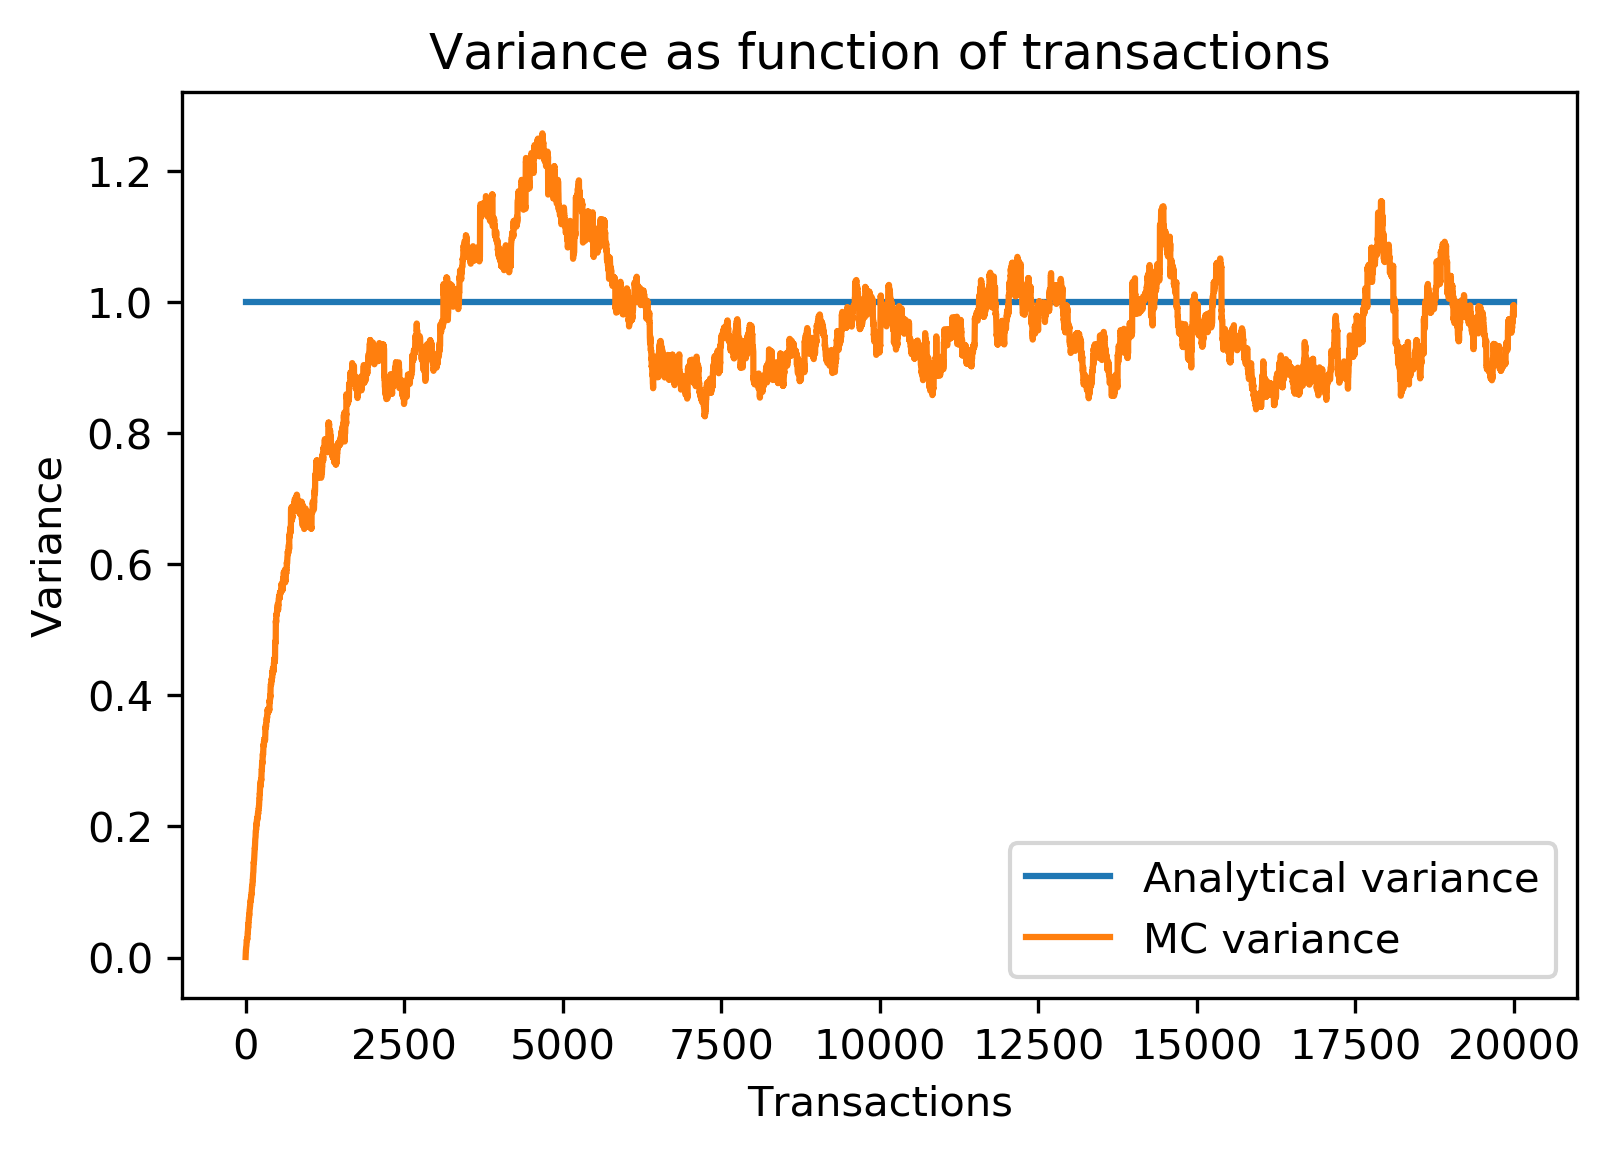
\includegraphics[width=0.5\textwidth]{figures/var_1000c_15000t.png}}
  \hfill
  \subfloat[Cycle analysis]{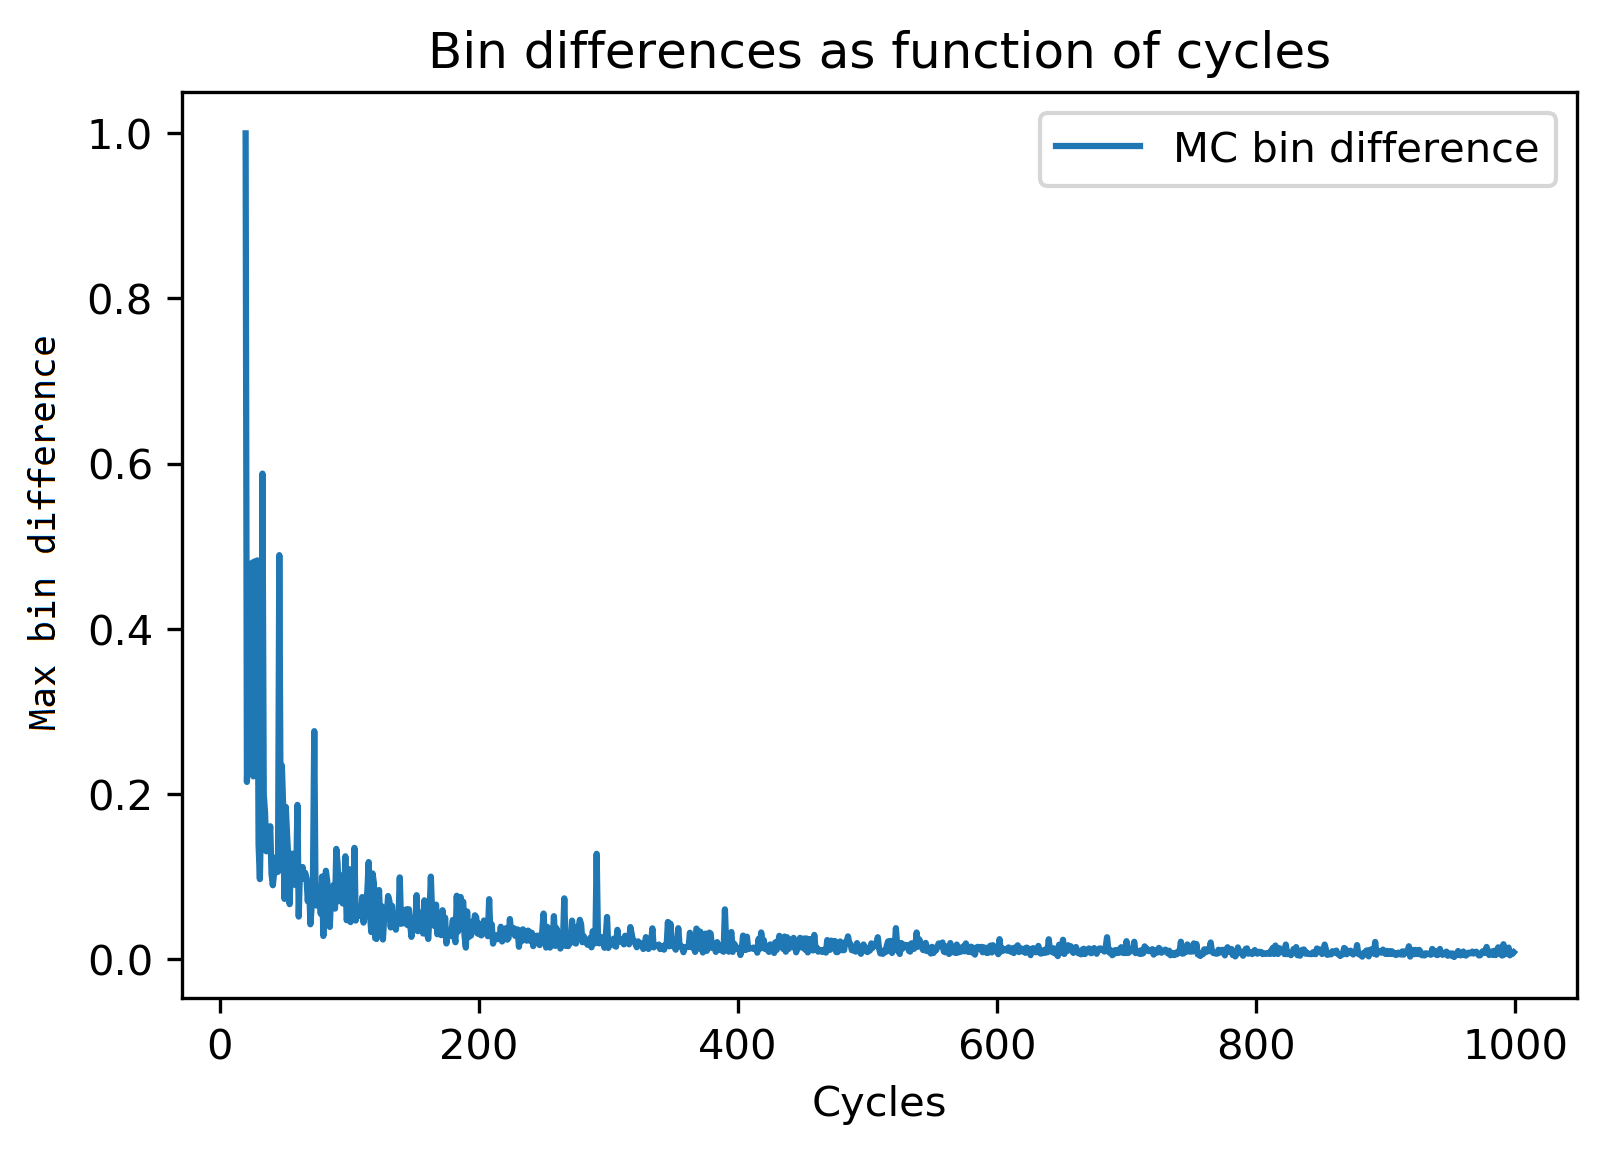
\includegraphics[width=0.5\textwidth]{figures/cycles_1000c_10000t.png}}
  \caption{Transaction and cycle analysis}
{\small Subfigure [a] was produced with $10^3$ cycles and subfigure [b] with $10^4$ transactions. Both with the values: $N = 500, m_0 = 1, \gamma = 0, \alpha = 0, \lambda = 0$. }
\end{figure}

Below are two figures that highlights the computed distribution of wealth in comparison with a Gibbs distribution of the system. We can safely say that they correspond to each other.
\begin{figure}[H]
  \subfloat[Distribution]{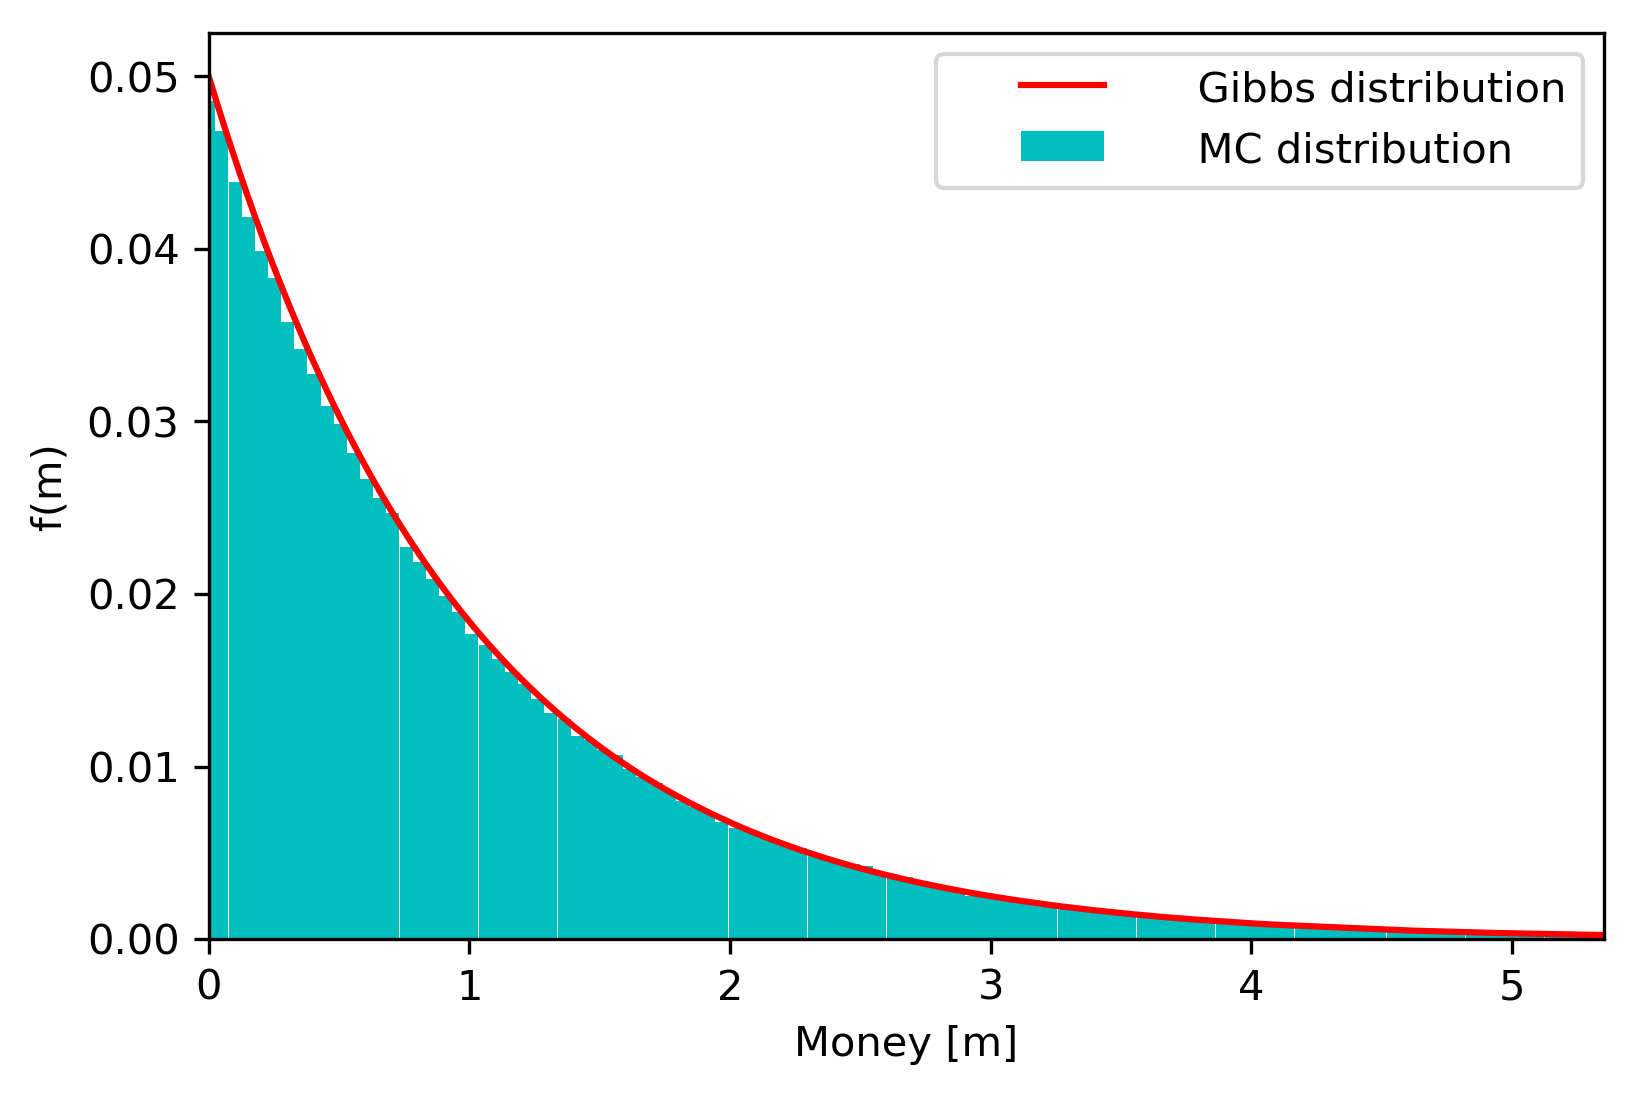
\includegraphics[width=0.5\textwidth]{figures/dist_1000c_10000t.png}}
  \hfill
  \subfloat[Log Distribution]{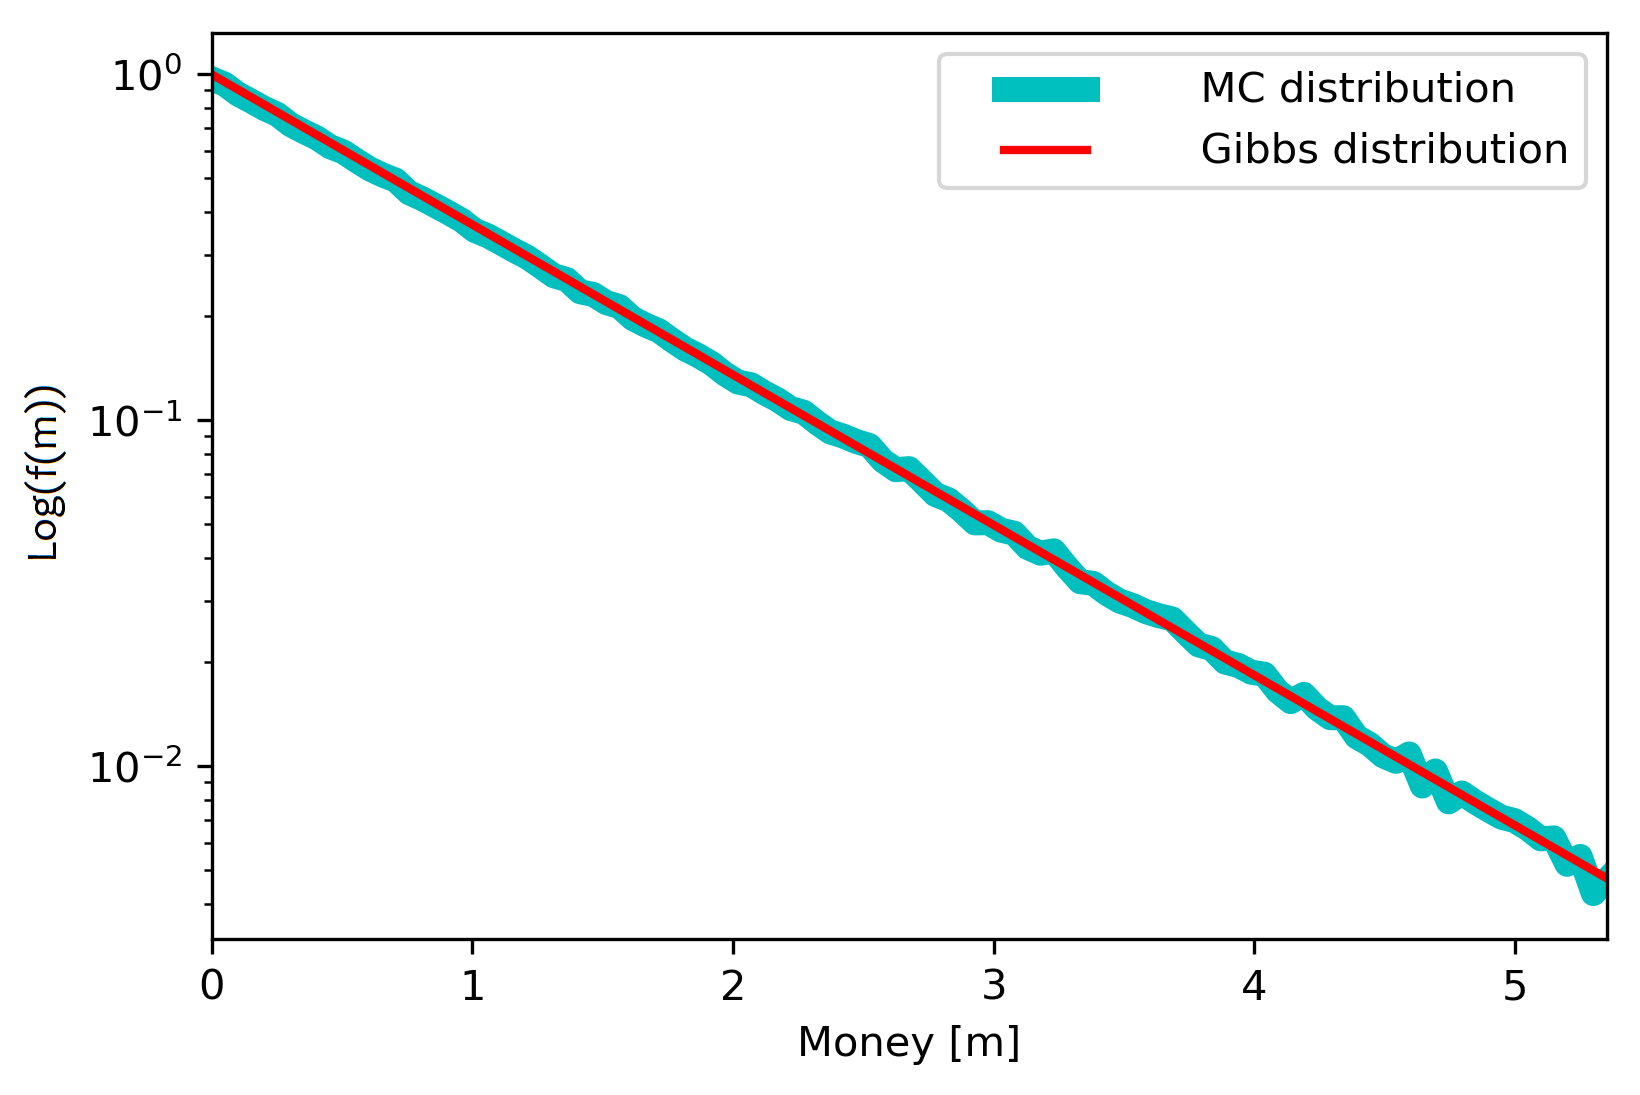
\includegraphics[width=0.5\textwidth]{figures/log_dist_1000c_10000t.png}}
  \caption{Recognizing the distribution}
{\small Both subfigures was produced with $10^3$ cycles and $10^4$ transactions. \\Both with the values: $N = 500, m_0 = 1, \gamma = 0, \alpha = 0, \lambda = 0$. }
\end{figure}


	\subsection{Saving factor included, Model [B]}
In this model the saving factor $\gamma$ is activated. The effect is that the distribution of money no longer correspond to a Gibbs distribution but rather a power law function, represented by the black boxes below. The power law function is found in Patriarca et al.[3]	
	
\begin{figure}[H]
	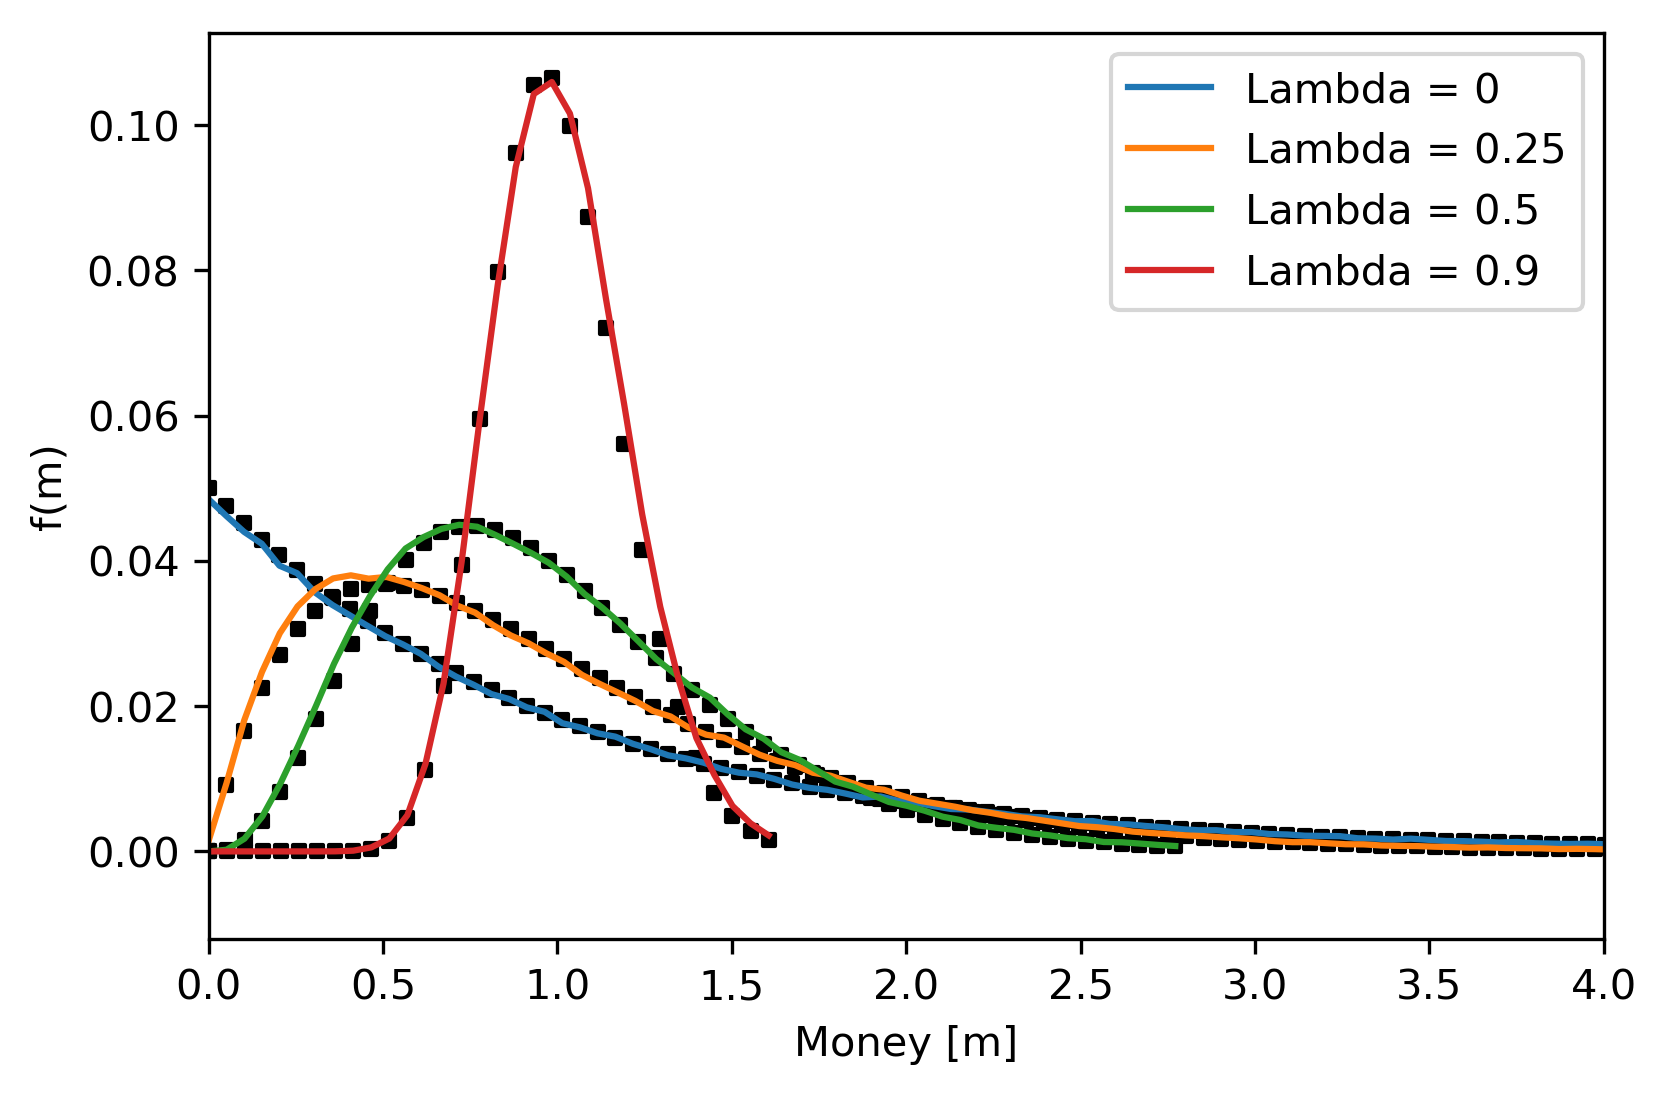
\includegraphics[scale=1]{figures/saving_1000c_100000t.png} 
	\caption{Equilibrium distributions for different saving factors [$\lambda$]}
{\small The figure was produced with $10^3$ cycles and $5*10^5$ transactions. \\With the values: $N = 500, m_0 = 1, \gamma = 0, \alpha = 0$. }
\end{figure}


Presented here are two end tails of the distribution with two different $\lambda$ values together with fitted power functions, calculated with the library scipy.

\begin{figure}[H]
  \subfloat[Log Distribution of tail, $\lambda=0.25$]{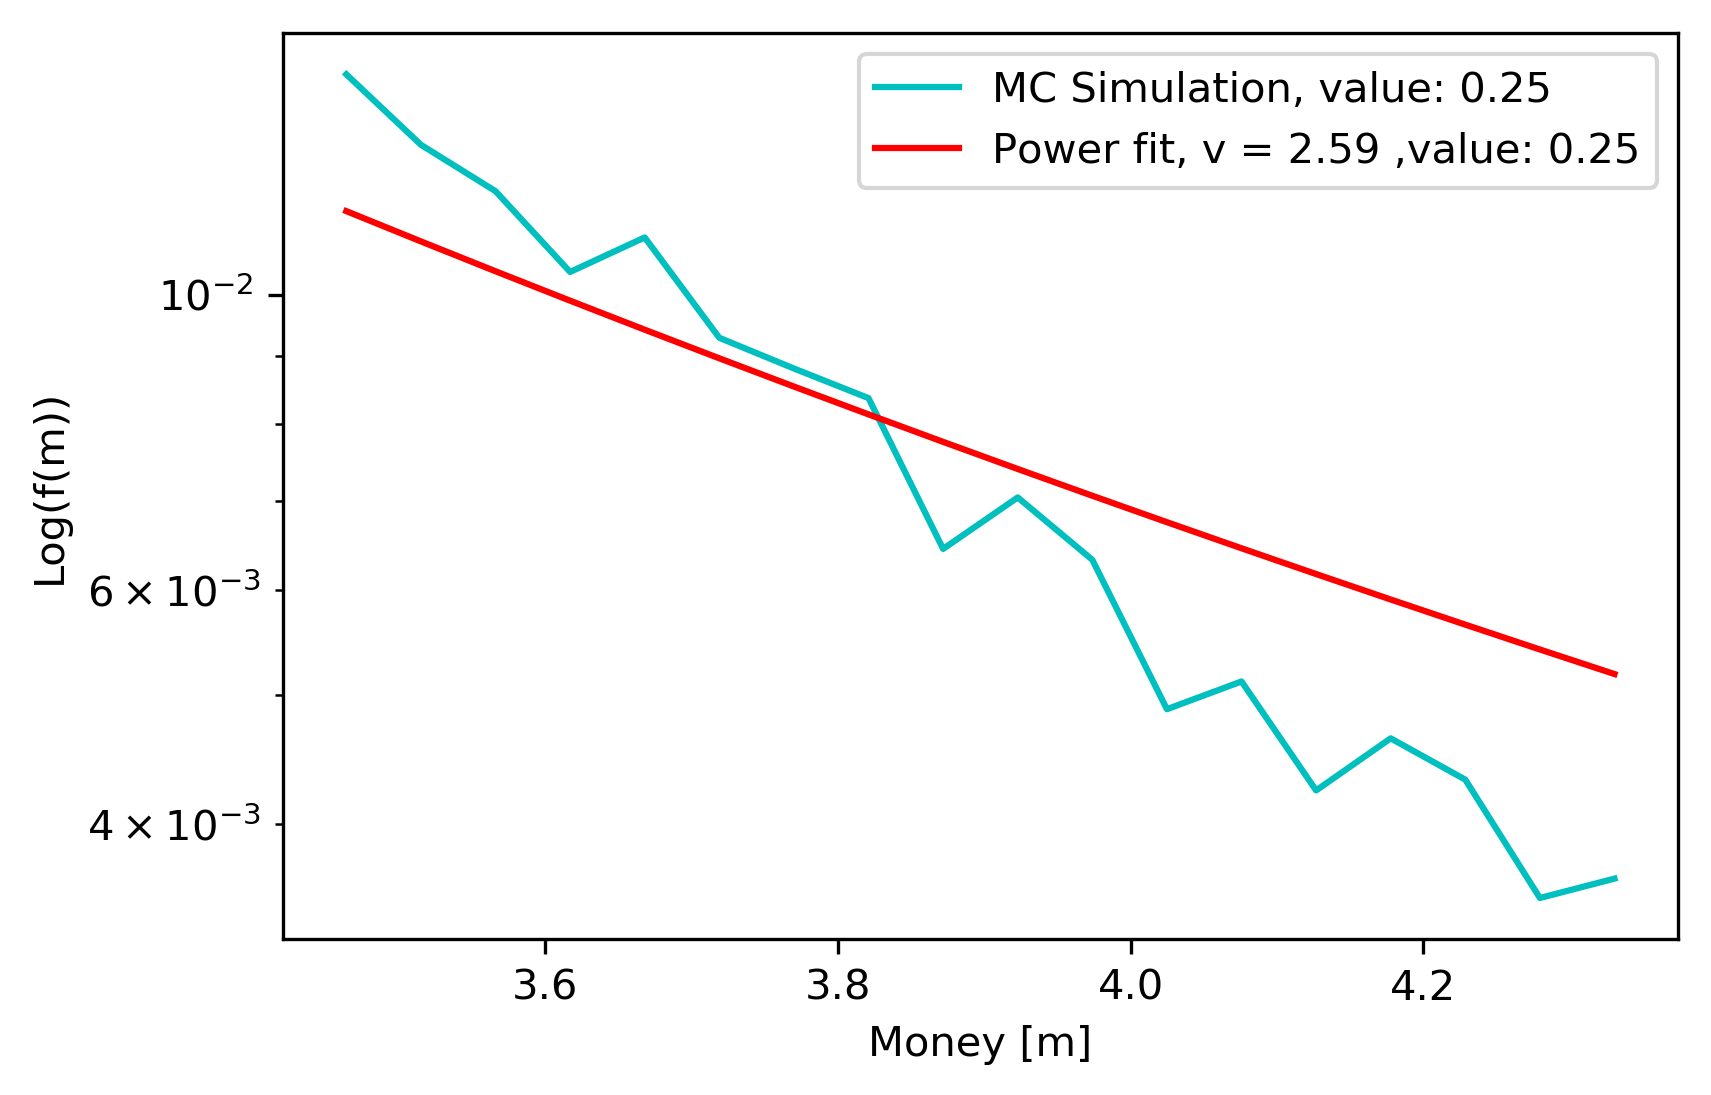
\includegraphics[width=0.5\textwidth]{figures/saving_tail_1000c_100000t_025.png}}
  \hfill
  \subfloat[Log Distribution of tail, $\lambda=0.50$]{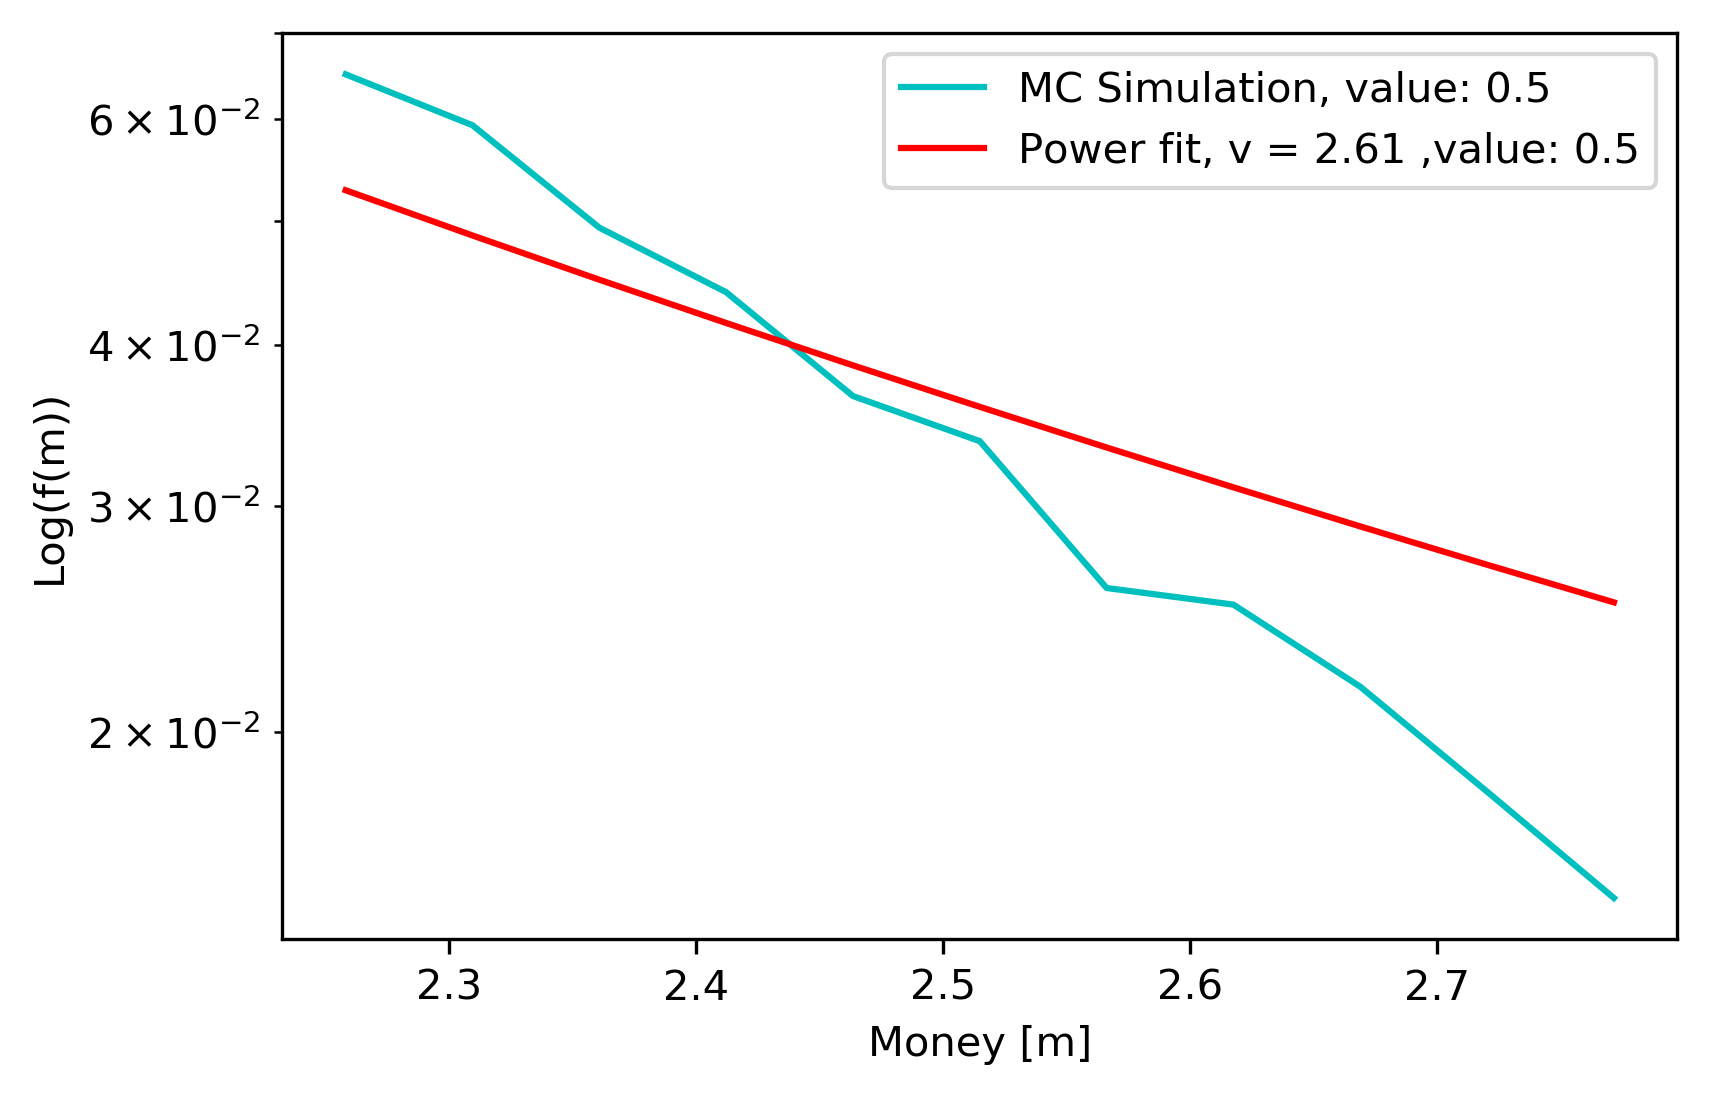
\includegraphics[width=0.5\textwidth]{figures/saving_tail_1000c_100000t_05.png}}
  \caption{End tail distribution}
{\small Both subfigures was produced with $10^3$ cycles and $5*10^5$ transactions. \\Both with the values: $N = 500, m_0 = 1, \gamma = 0, \alpha = 0$. \\End tail is defined as the wealthiest 20\% }
\end{figure}


	\subsection{Relationship factor included, Model [C]}
In this model the relationship factor $\alpha$ is included. The effect is that the inequality increases as the end tail grows in wealth, as can be seen below.
	
\begin{figure}[H]
	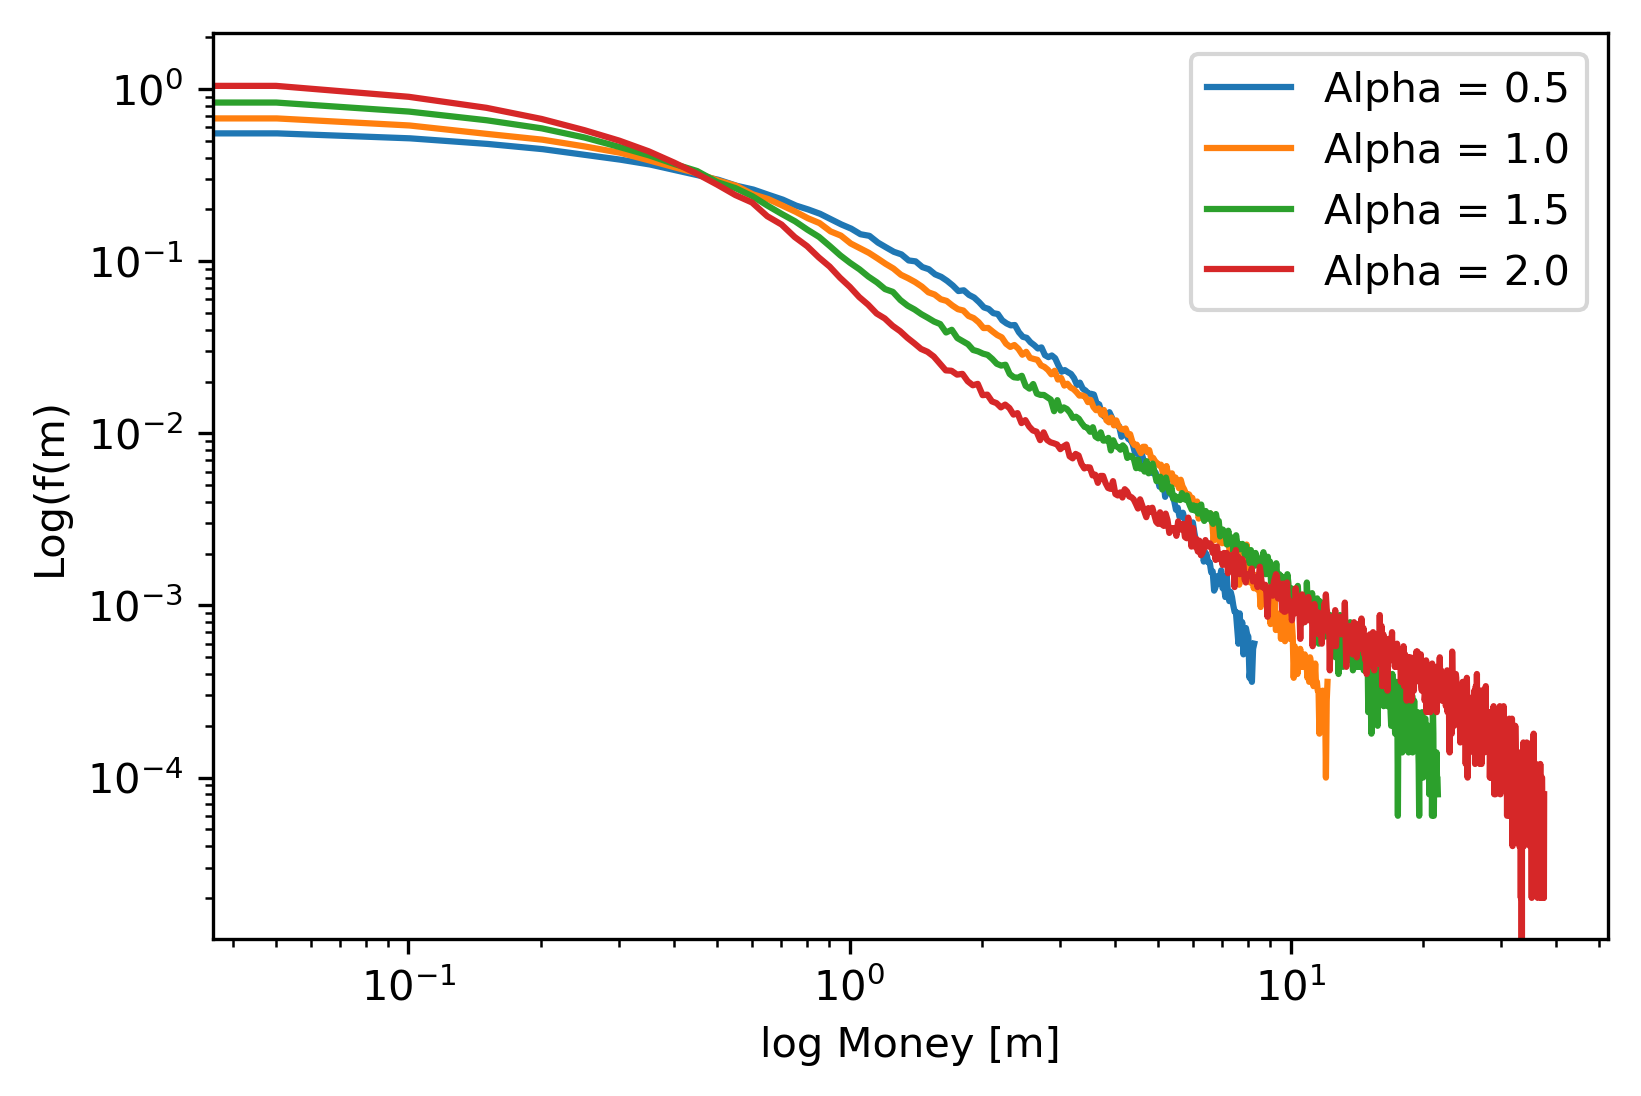
\includegraphics[scale=1]{figures/relationship_1000c_200000t.png} 
	\caption{Equilibrium distributions for different relationship factors $\alpha$}
{\small The figure was produced with $10^3$ cycles and $2*10^5$ transactions. \\With the values: $N = 500, m_0 = 1, \gamma = 0, \lambda = 0$. }
\end{figure}

We also present two graphs of the end tail and the fitted power functions, which clearly demonstrate the Pareto distribution for $\alpha>1$

\begin{figure}[H]
  \subfloat[Log Distribution of tail, $\alpha=0.5$]{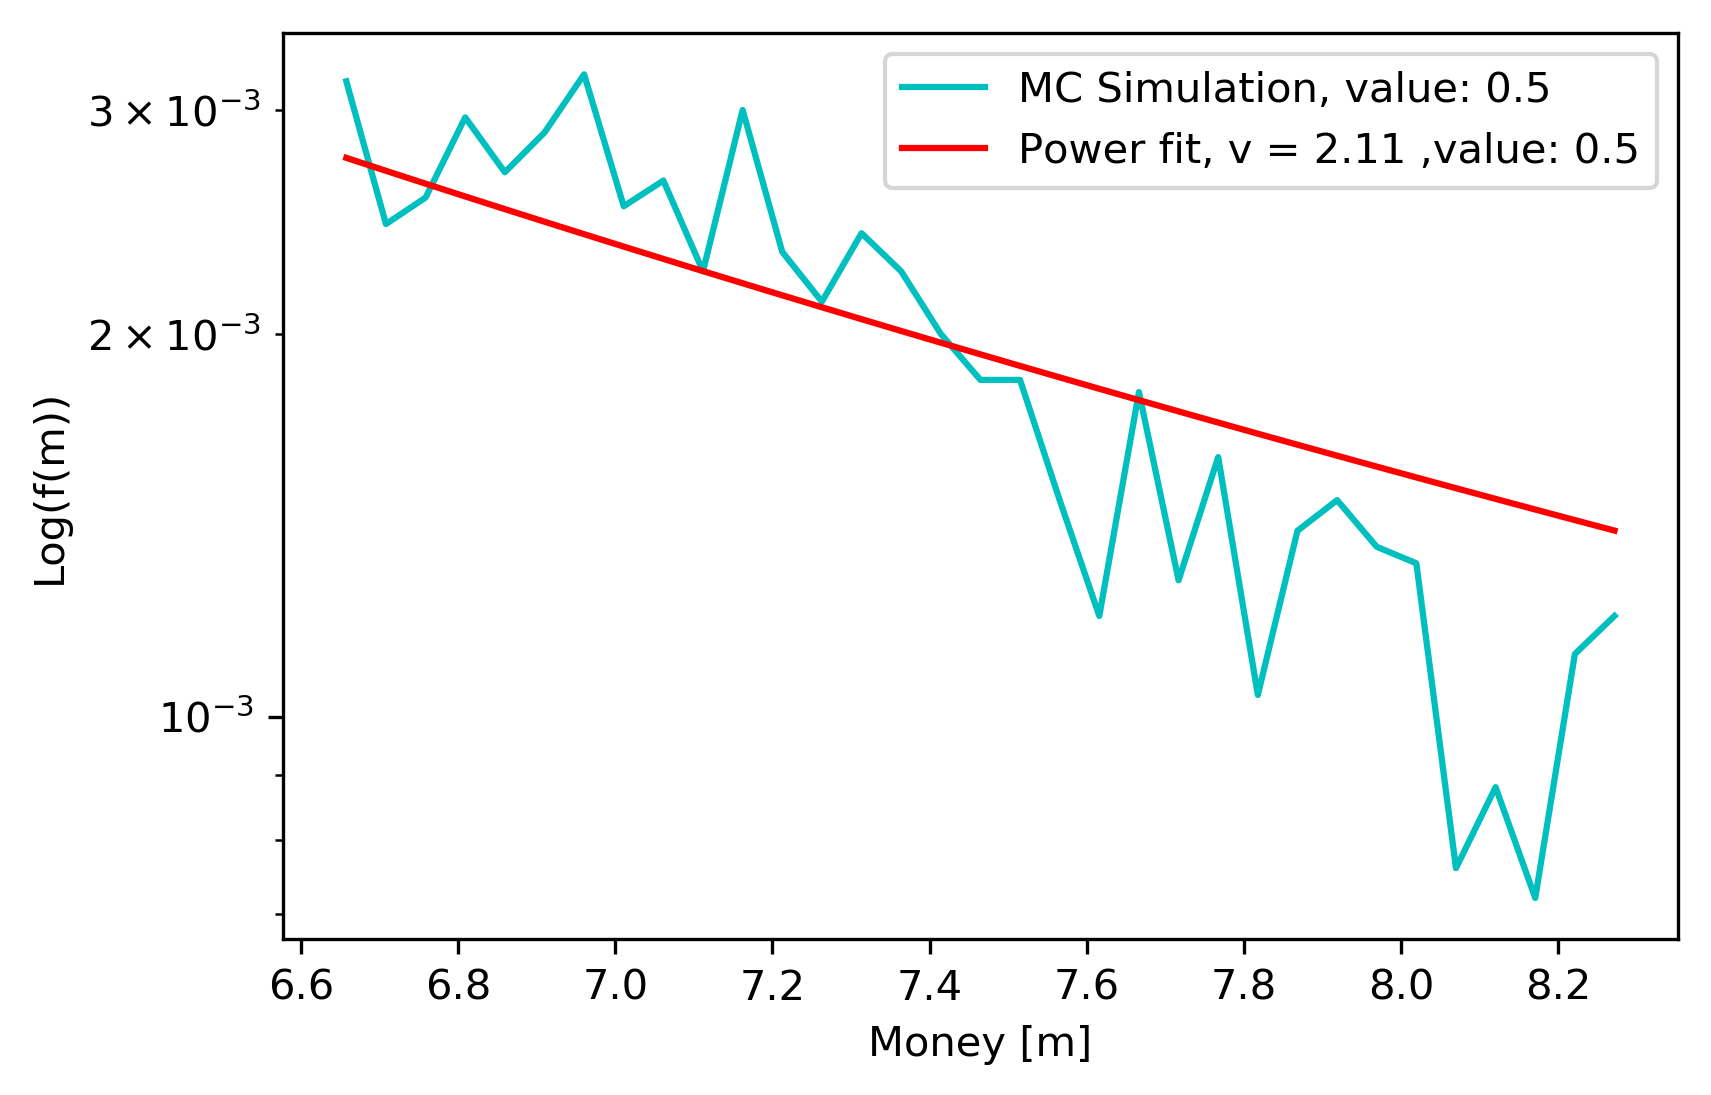
\includegraphics[width=0.5\textwidth]{figures/relationship_tail_1000c_200000t_05.png}}
  \hfill
  \subfloat[Log Distribution of tail, $\alpha=1.5$]{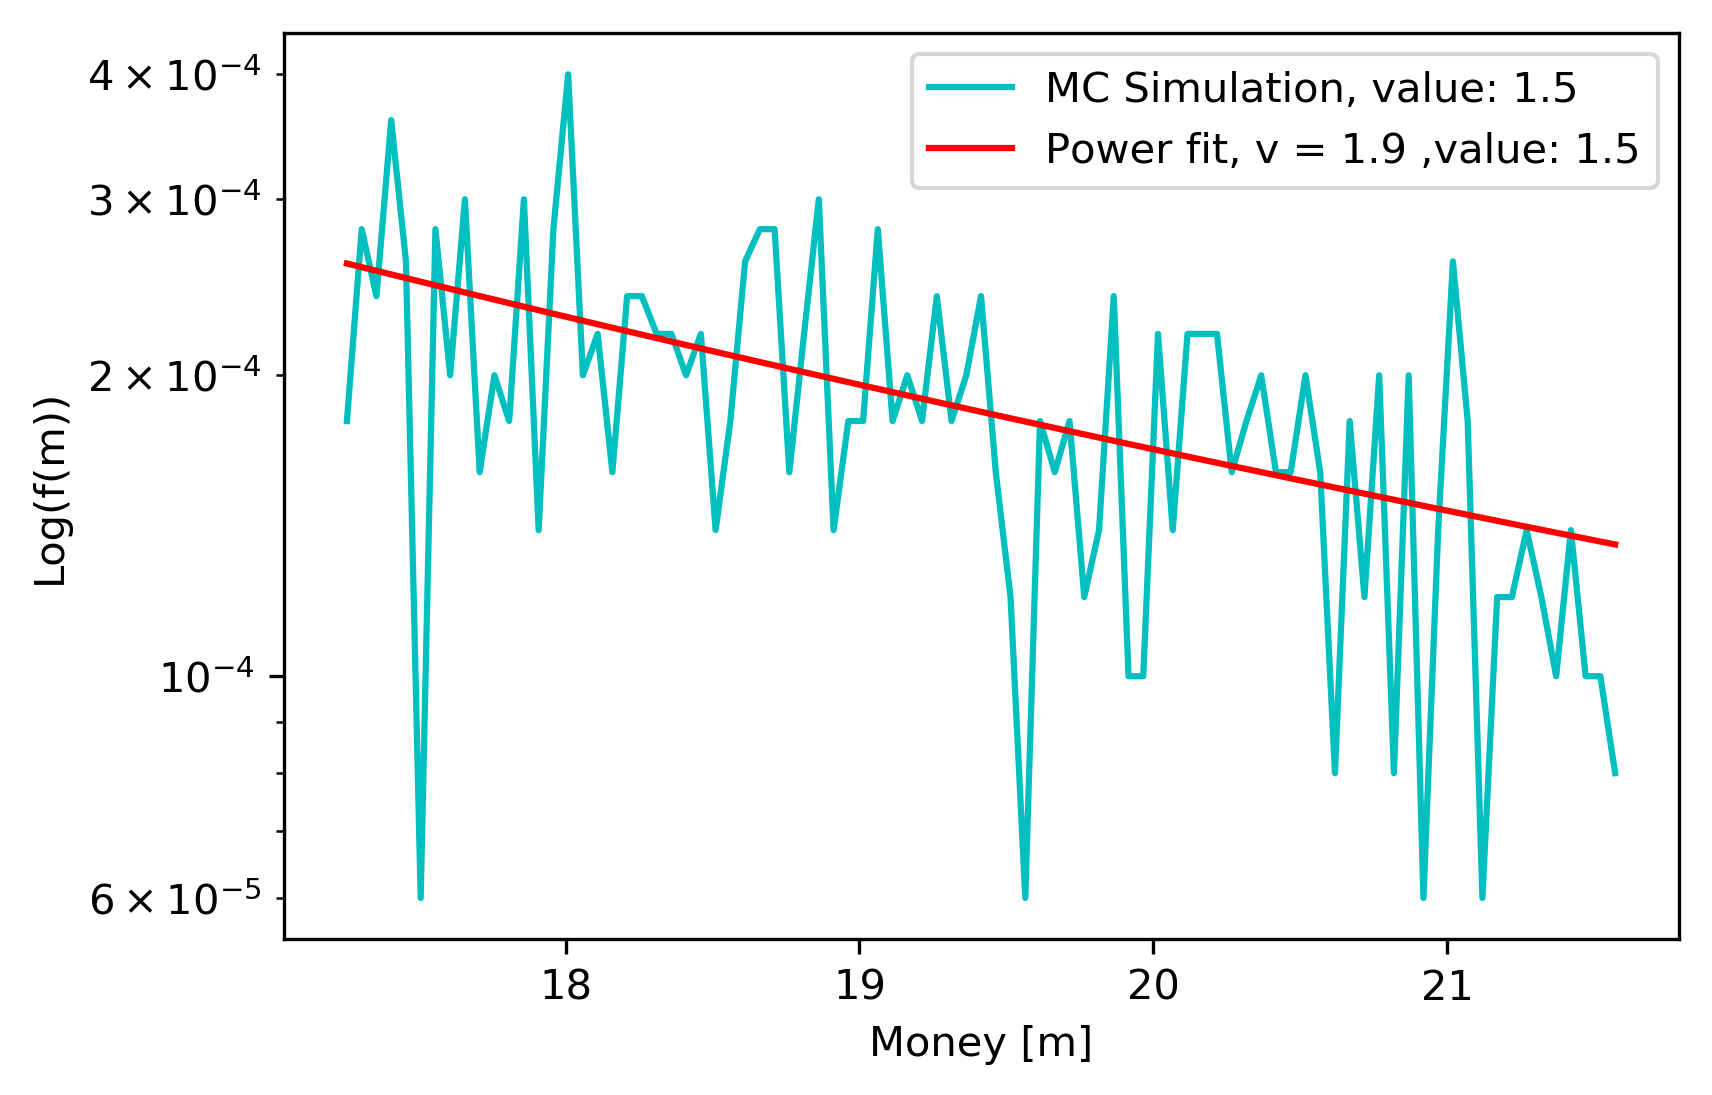
\includegraphics[width=0.5\textwidth]{figures/relationship_tail_1000c_200000t_015.png}}
  \caption{End tail distribution}
{\small Both subfigures was produced with $10^3$ cycles and $2*10^5$ transactions. \\Both with the values: $N = 500, m_0 = 1, \gamma = 0, \lambda = 0$. \\End tail is defined as the wealthiest 20\% }
\end{figure}

	\subsection{Memory factor included, Model [D]}
In this model the relationship factor $\gamma$ is activated. These results shows how the $\gamma$	factor reduces the effect of the strong $\alpha$ factor, hence decreasing the inequality.
	
\begin{figure}[H]
	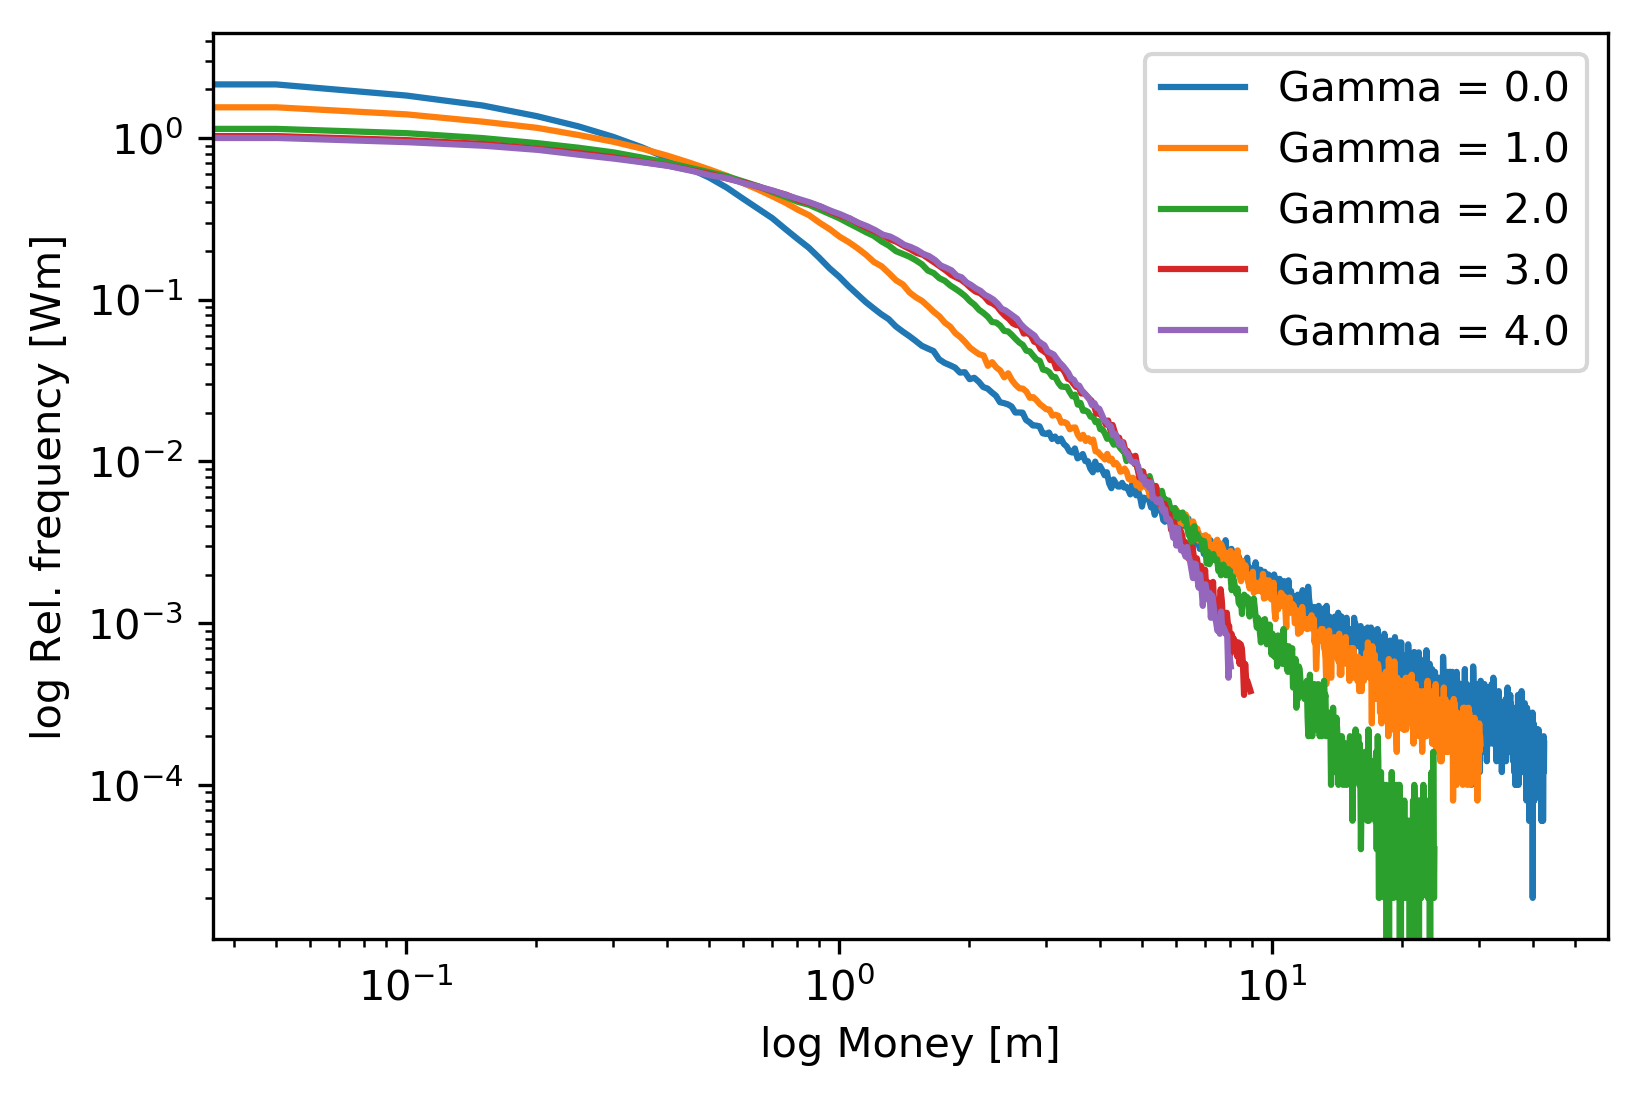
\includegraphics[scale=1]{figures/relationship_mem_1000c_1000000t_nosave_a2.png} 
	\caption{Equilibrium distributions for different relationship factors $\gamma$}
{\small The figure was produced with $10^3$ cycles and $10^6$ transactions. \\With the values: $N = 500, m_0 = 1, \alpha = 2, \lambda = 0$. }
\end{figure}
Included is once again two end tails and their corresponding fits.
\begin{figure}[H]
  \subfloat[Log Distribution of tail, $\gamma=1.0$]{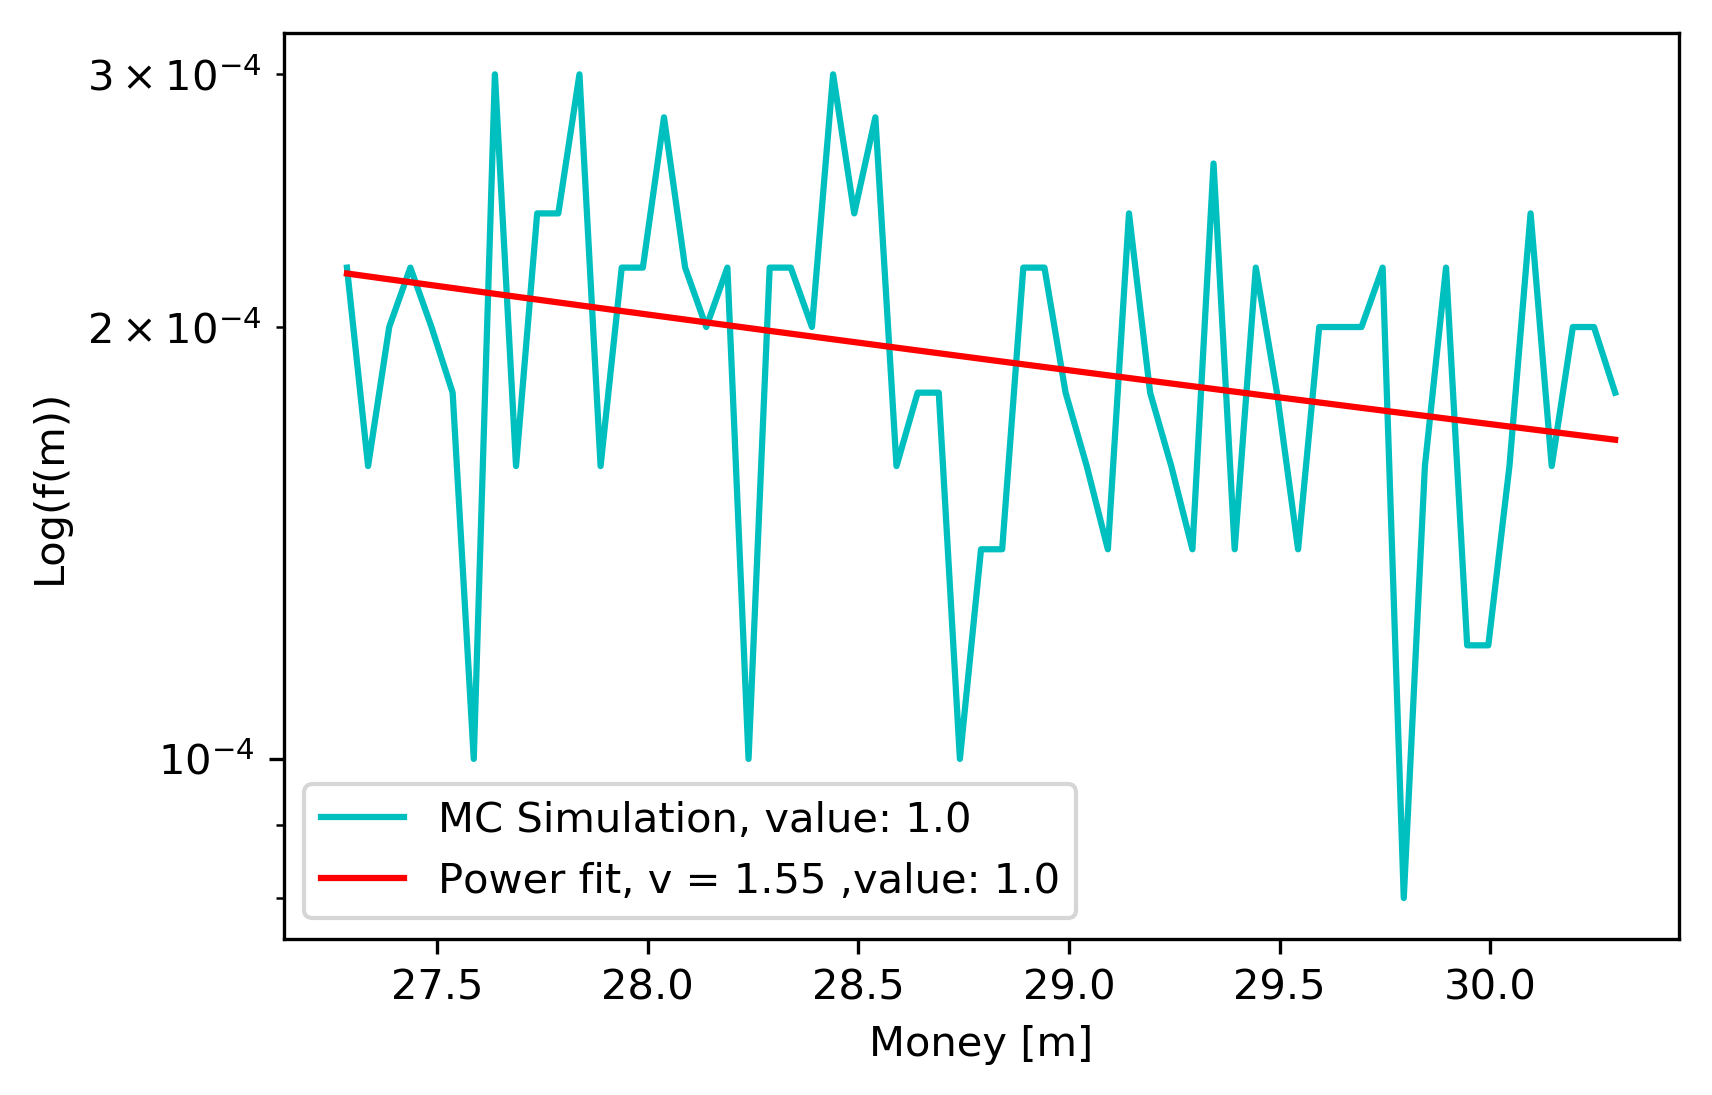
\includegraphics[width=0.5\textwidth]{figures/relationship_mem_tail_1000c_1000000t_nosave_a2_g1.png}}
  \hfill
  \subfloat[Log Distribution of tail, $\gamma=2.0$]{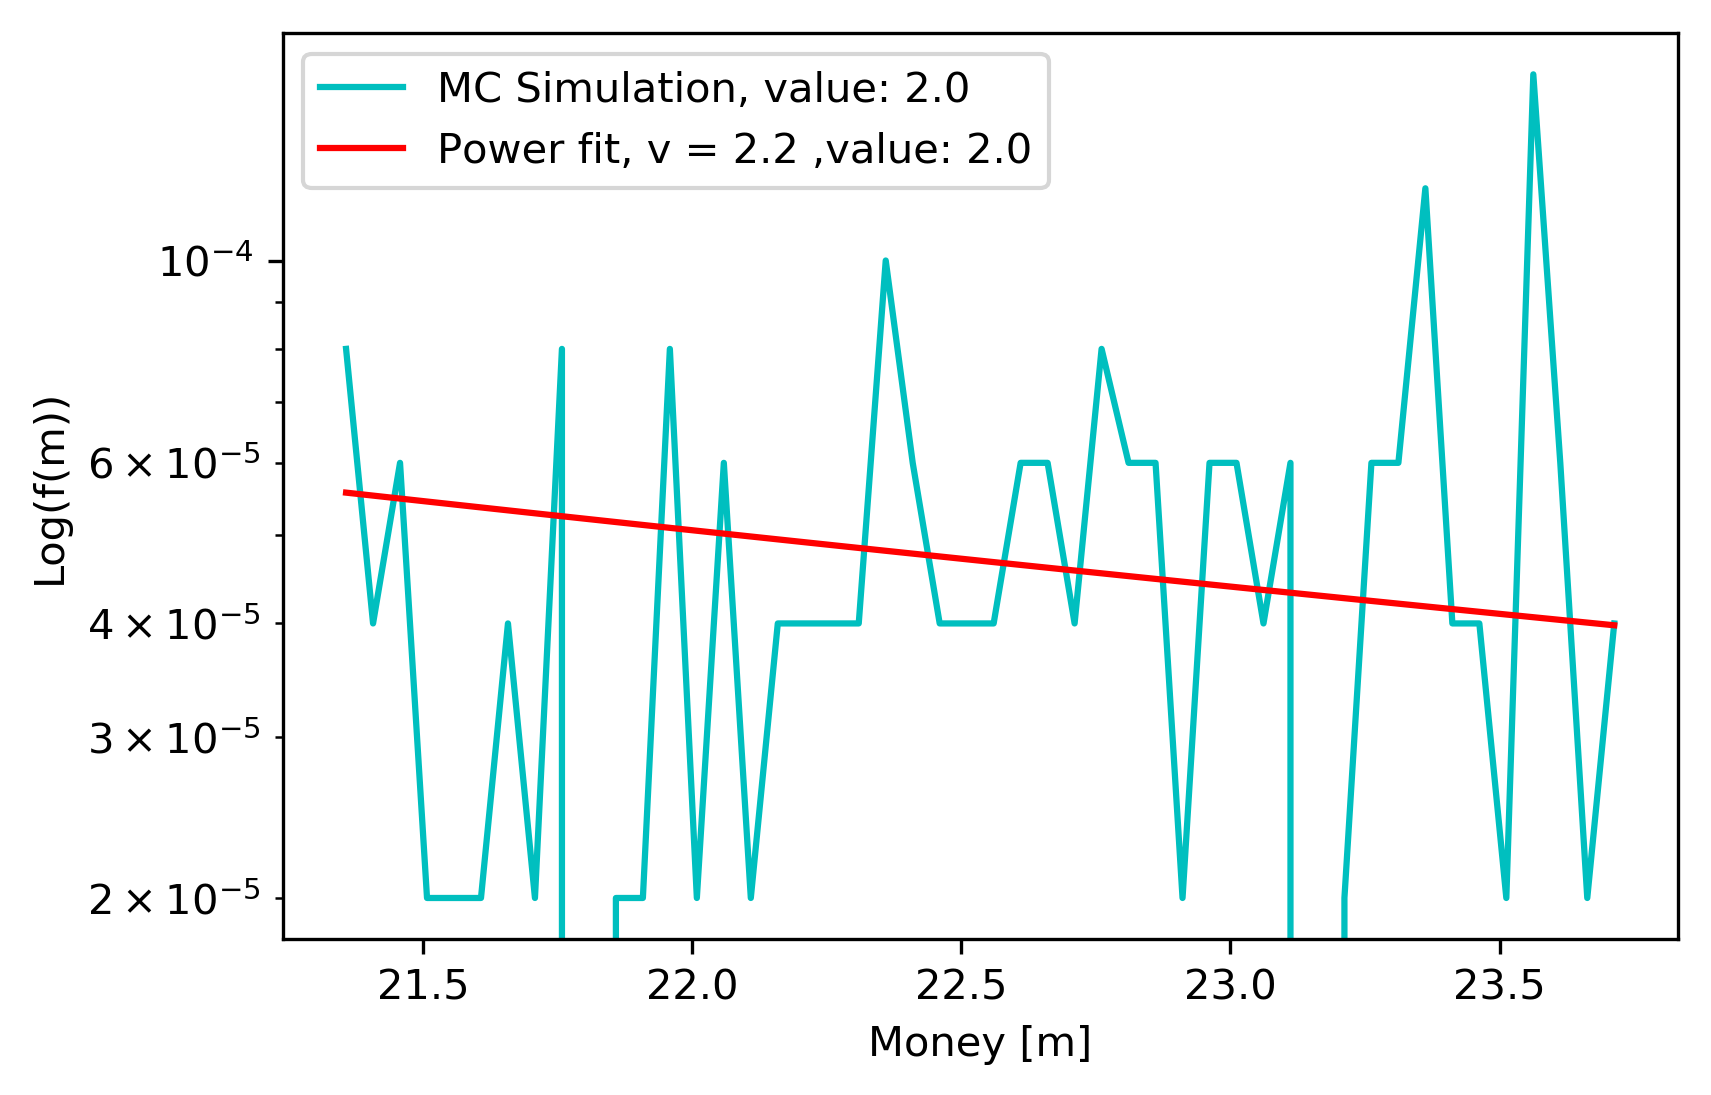
\includegraphics[width=0.5\textwidth]{figures/relationship_mem_tail_1000c_1000000t_nosave_a2_g2.png}}
  \caption{End tail distribution}
{\small Both subfigures was produced with $10^3$ cycles and $10^6$ transactions. \\Both with the values: $N = 500, m_0 = 1, \gamma = 0, \lambda = 0, \alpha = 2$. \\The end tail is defined as the wealthiest 20\% }
\end{figure}

\section{Discussion}
A chosen equilibrium point can be drawn from figure [1], where there is evident that the variance begin to oscillate around the analytical value when the number of needed transactions are reached. It is also clear that the system stabilizes after a certain number of cycles. During the progress of the project, it was discovered that the number of cycles seems to govern the noise of the system. But it is the number of transactions that is of critical importance for the ability to analyse a fully relaxed system. The number of transactions and cycles needed for obtaining a fully relaxed state seems to vary with the factors included as well.
\\
\par
Model [A] confirm that the algorithm is working properly as the distribution clearly correspond with the expected Gibbs distribution, see figure [2]. By introducing the saving factor in Model [B], we can see that the system no longer follows a Gibbs distribution, but rather a Poisson distribution. Figure [3] presents the results of Model [B], which corresponds well with figure [1] from Patriarca et al.[3] It can also be seen that the distribution follows the power law function presented by Patriarca et al.[3]. The implication of the saving factor is highlighted when comparing the blue curve $\lambda = 0$ and the red curve $\lambda = 0.9$. The inequality is lower for the red curve, compared to the blue, which is the same as Model [A], where only a few possesses the majority of the the wealth.
\\
\par
Figure [4] is an attempt to fit the end tail, it is not an optimal fit, as it requires a fully relaxed system which was not obtained with only $5*10^5$ transactions. But, the indications of a power law tail is there. It was generally observed throughout the project that the Pareto exponent decreased towards a more expected range with a higher amount of transactions. However, the computational time for $10^7$ transactions and $10^3$ cycles was estimated to a staggering 25-30 hours.
\\
\par
In Model [C] we add the relationship factor $\alpha$ in order to reflect figure [1] from the Goswami et al.[4]. Our figure [5] correspond well. The figure also highlight how the uncertainty increases as we move towards the end tail. This can simply be explained by the fewer individuals reaching these bins, creating some fluctuation. The tail analysis in figure [6] strongly indicate that for $\alpha >> 1$ the tail can be properly described by a power law. Regarding the implication on the distribution, a higher $\alpha$ value seems to increase the wealth of the end tail, hence increasing the inequality. The results of adding $\lambda = 0.5$ into this model lowers the inequality further, as expected. However, the power law tail still holds well, see appendix [1].
\\
\par
In Model [D] the memory factor $\gamma$ is added for reflecting figure [5] from Goswami et al.[4]. It was hard to reproduce this figure as the values given by Goswami et al. are sparse and our number of transactions is low. Noted shall that $\gamma = 1$ seems to approach $\gamma = 0$ as it evolves into a more or less straight line, while $\gamma = [3,4]$ has barley evolved. So with enough transactions there is a probability that the red, green and purple curves straightens out and maybe end up coincide with each other in a fully relaxed state.
\\
\par
Regarding the implication of $\gamma$ it can be seen that the inequality simply decreases as the individuals tend to trade in small clusters, hence limiting the flow of wealth. We also activated the saving factor $\lambda$ in this model. The effect was similar to the model [C] case with added $\lambda$, see appendix[2]. 

\section{Conclusion}
The Monte Carlo algorithm successfully performed the computation and allowed us to analyse the economical evolution of a closed system. The drawback for the method is the computational time needed.
\\
\par
The saving factor $\lambda$ contribute with a more equally distribution of wealth and shortening the end tail. We can conclude that the relationship factor [$\alpha$] robustly increases the wealth of the richest. It is also concluded that for $alpha >> 1$ a tail with Pareto distribution described by a power law will be the case. And finally, by adding the memory factor $\gamma$ the system tend to trade in small clusters, leading to a restricted flow of wealth. The implication is that the inequality decreases. The main conclusion is that the power law tail seems to hold even if we keep inserting new factors that alter the overall distribution. And so, the claimed Pareto distribution for the end tail can be concluded for this study as well.
\\
\par
Future investigation is recommended to first run the experiments with at least $10^7$ transactions, as it will yield more accurate tail data. Especially for the models containing the $\gamma$ factor. Alternative factors to add could be a debt factor and an interest factor which would reflect the real world scenario even more. It would be of particular interest to observe the evolution of the end tail, as a function of overspending individuals.

\section{Appendix}

\textbf{1. The addition of $\lambda$ into Model [C]}
\begin{figure}[H]
	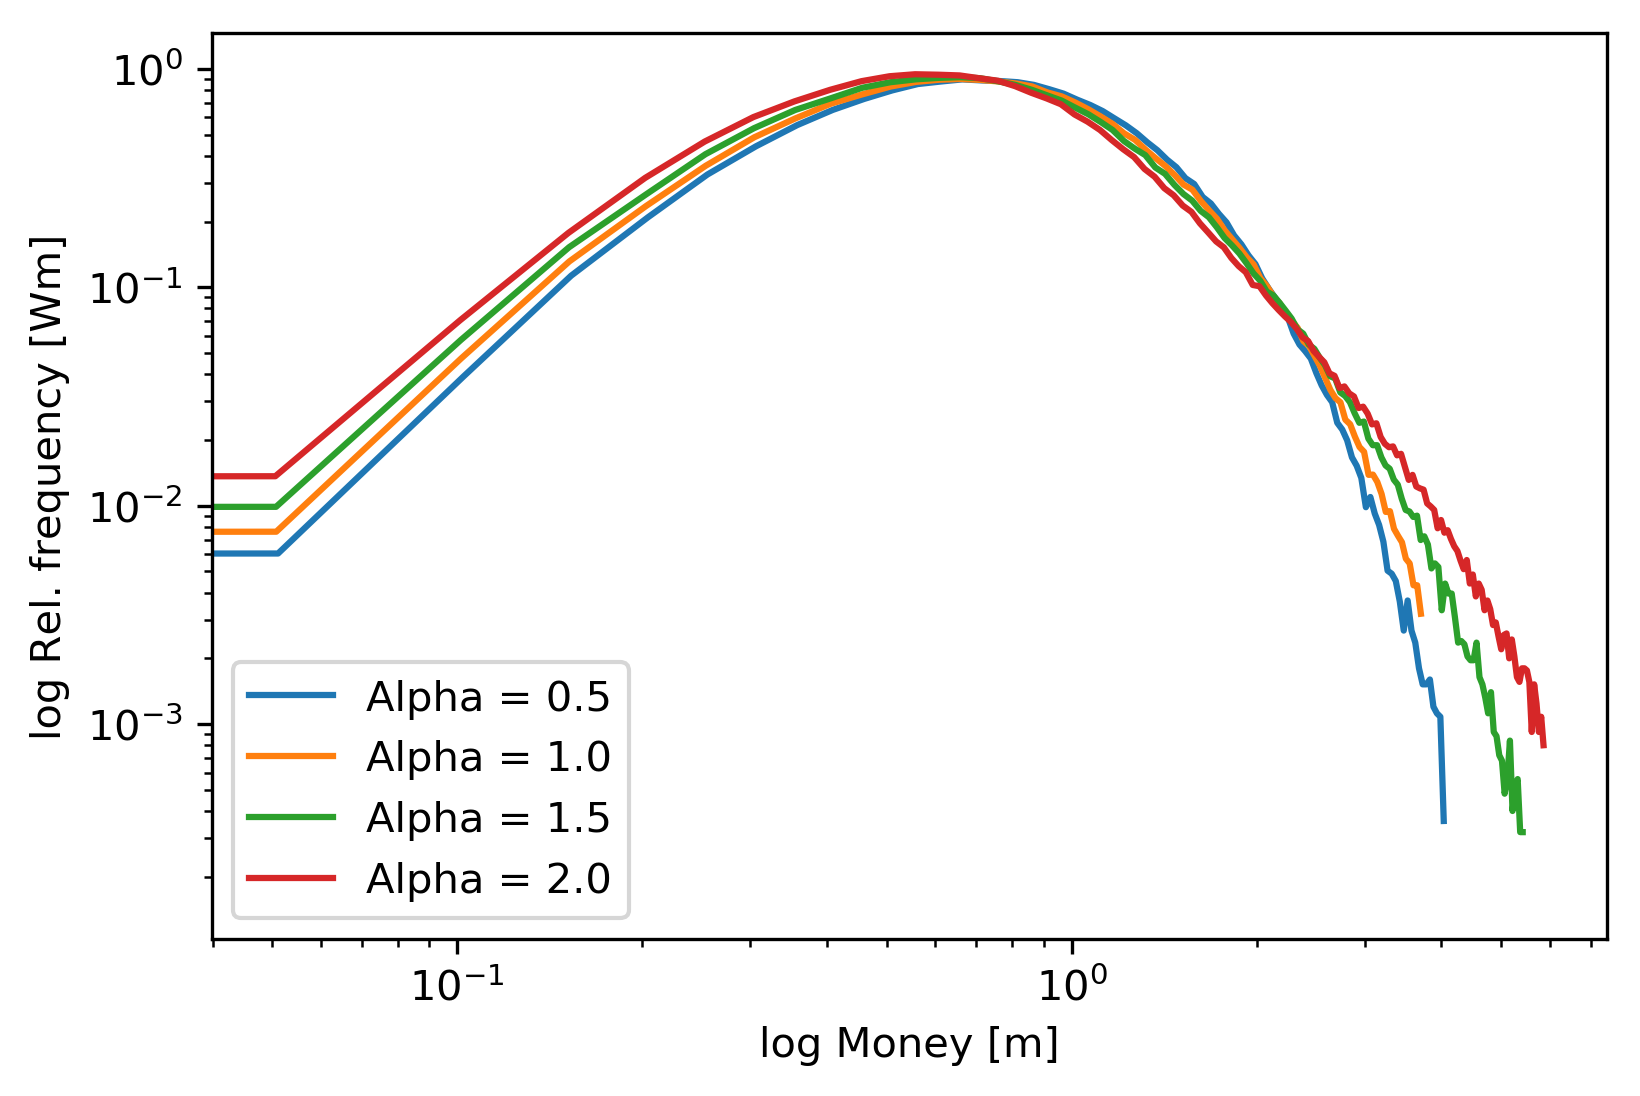
\includegraphics[scale=1]{figures/relationship_save_1000c_200000t.png} 
	\caption{Equilibrium distributions for different relationship factors [$\alpha$]}
{\small The figure was produced with $10^3$ cycles and $2*10^5$ transactions. \\With the values: $N = 1000, m_0 = 1, \gamma = 0, \lambda = 0.5$. }
\end{figure}

\begin{figure}[H]
  \subfloat[Log Distribution of tail, $\alpha=0.5$]{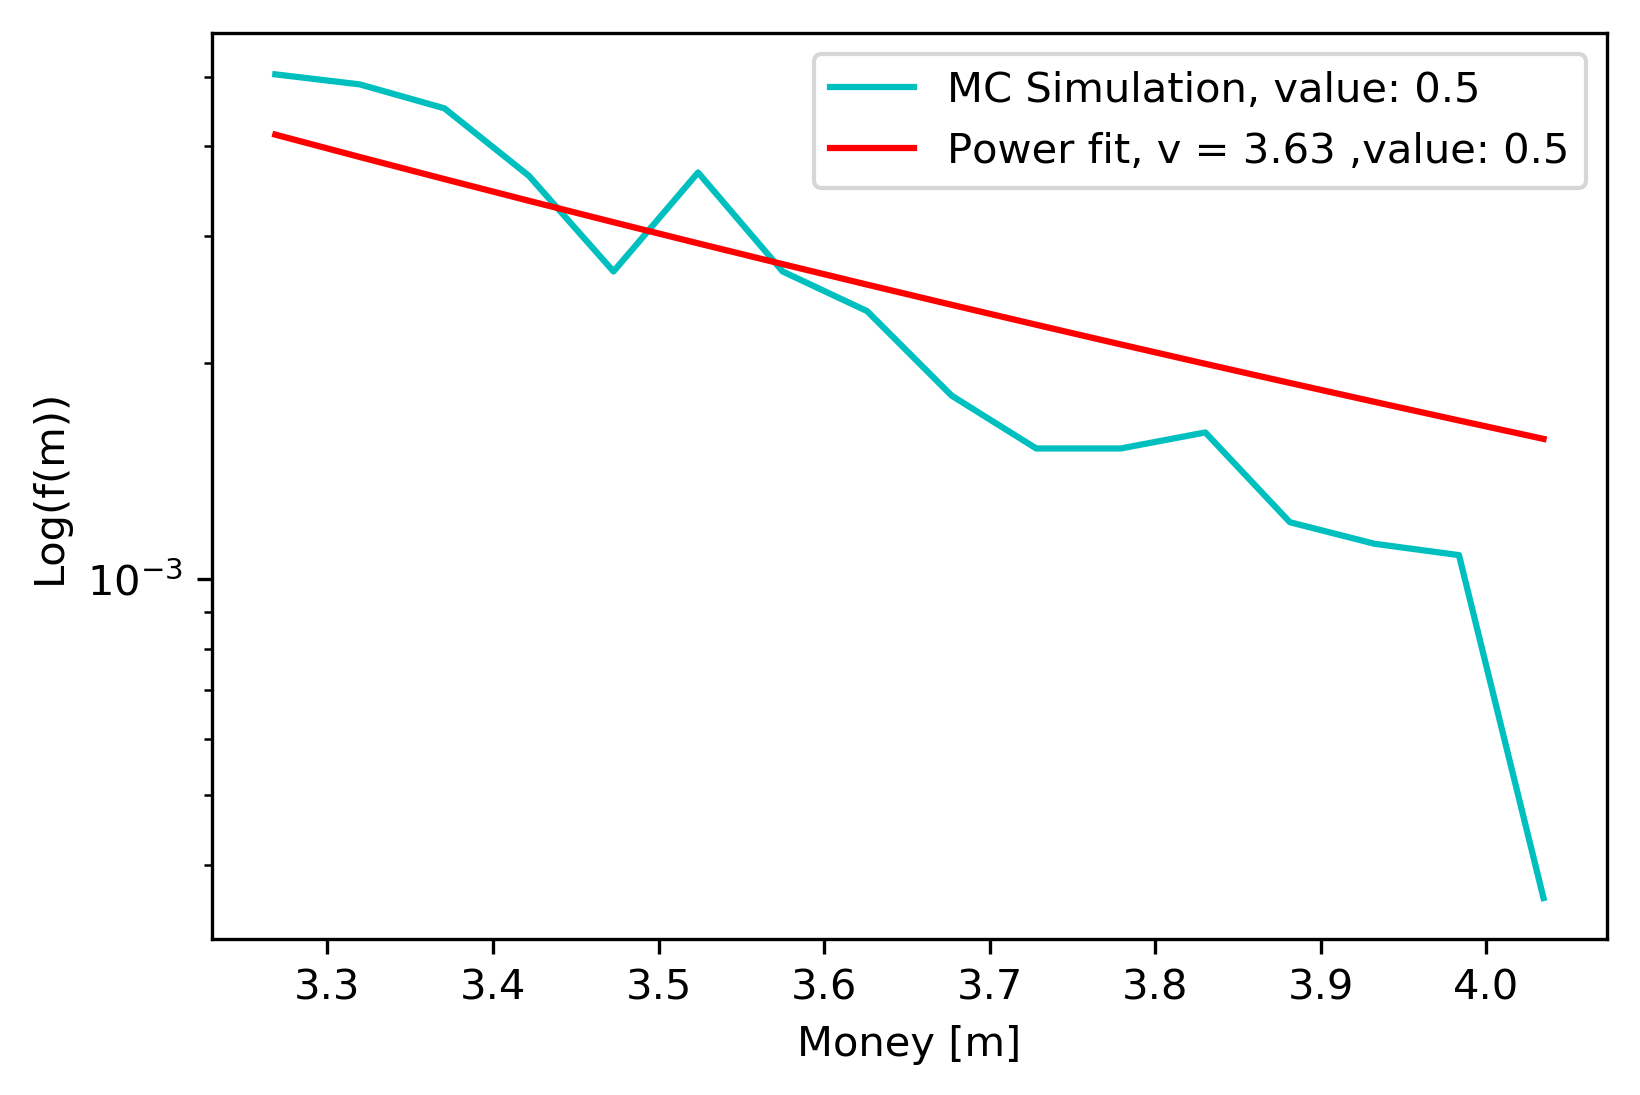
\includegraphics[width=0.5\textwidth]{figures/relationship_save_tail_1000c_200000t_005.png}}
  \hfill
  \subfloat[Log Distribution of tail, $\alpha=1.5$]{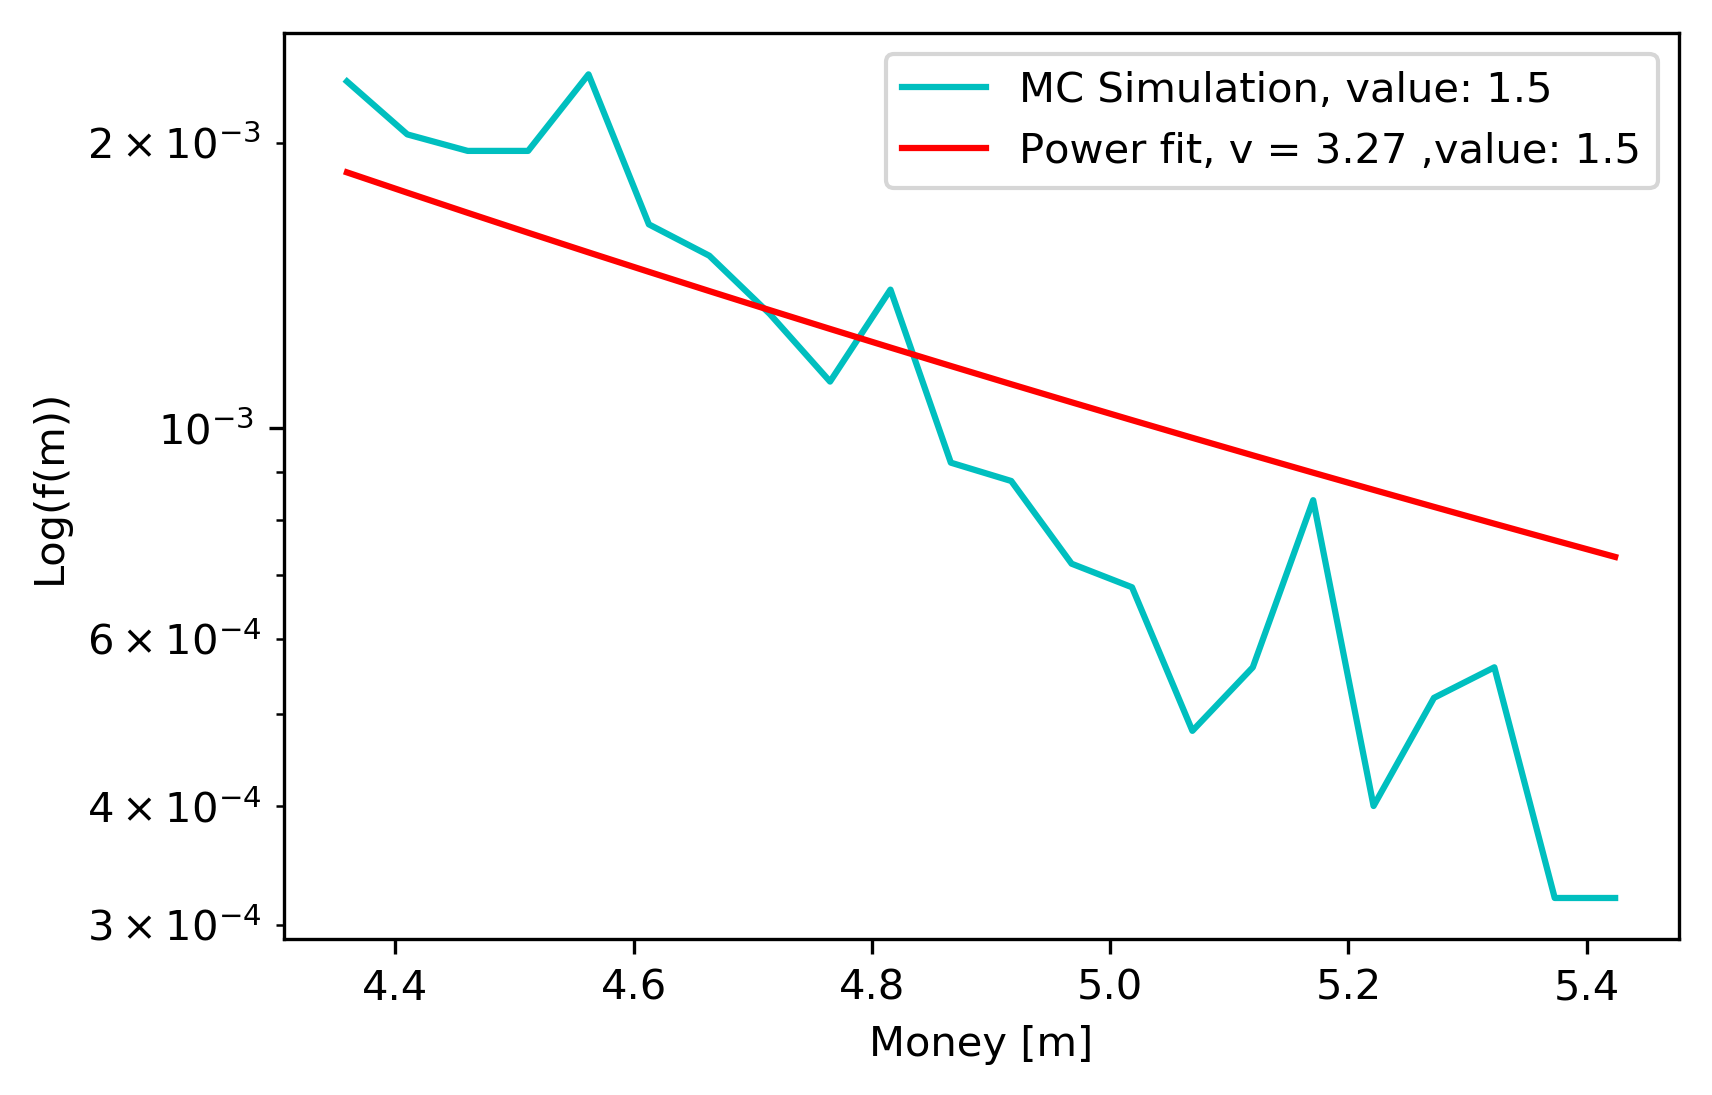
\includegraphics[width=0.5\textwidth]{figures/relationship_save_tail_1000c_200000t_015.png}}
  \caption{End tail distribution}
{\small Both subfigures was produced with $10^3$ cycles and $2*10^5$ transactions. \\Both with the values: $N = 1000, m_0 = 1, \gamma = 0, \lambda = 0.5$. \\The end tail is defined as the wealthiest 20\% }
\end{figure}

\textbf{2. The addition of $\lambda$ into Model [D]}
\begin{figure}[H]
	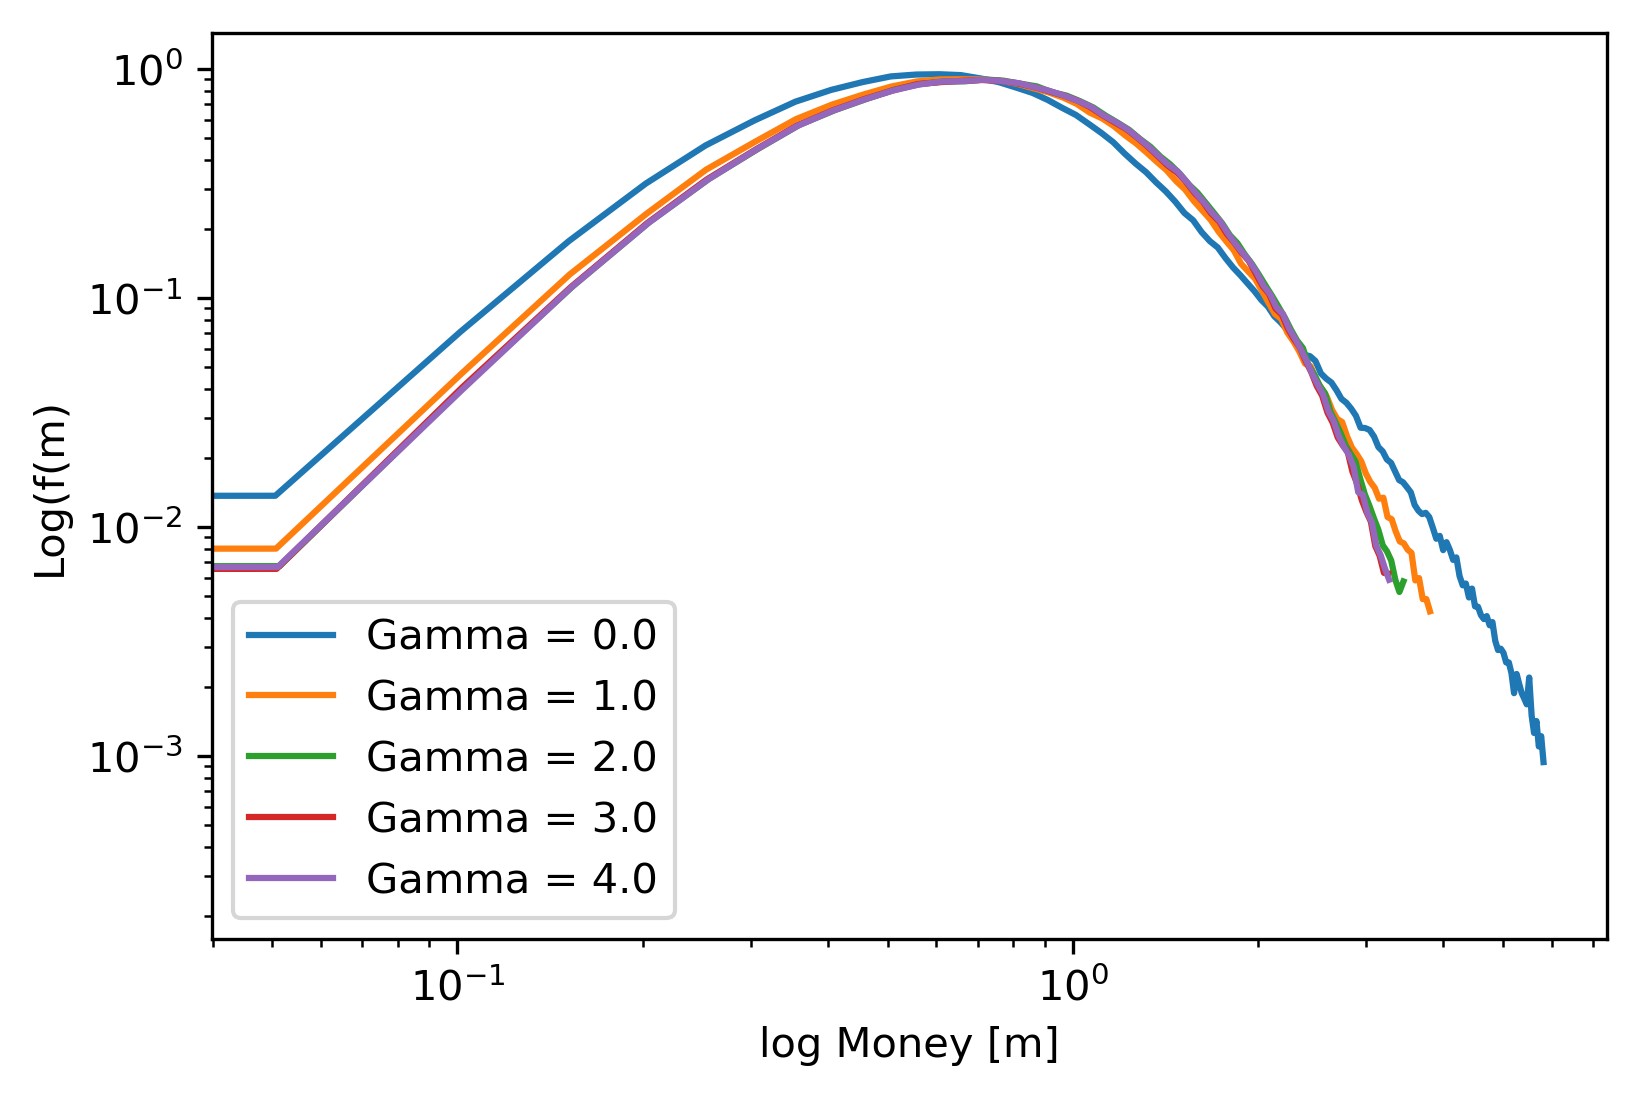
\includegraphics[scale=1]{figures/relationship_mem_save_1000c_200000t.png} 
	\caption{Equilibrium distributions for different memory factors [$\alpha$]}
{\small The figure was produced with $10^3$ cycles and $5*10^5$ transactions.
\\With the values: $N = 500, m_0 = 1, \alpha = 2, \lambda = 0.5$. }
\end{figure}

\textbf{Access to all material can be found at:}
\\
\url{https://github.com/silverberg89/FYS4150/blob/master/Project5/}

\begin{thebibliography}{9}
    \bibitem{VP}  Vilfredo Pareto. 1897. Cours d’economie politique. [ONLINE] Available at: http://www.institutcoppet.org/2012/05/08/cours-deconomie-politique-1896-de-vilfredo-pareto. [Accessed 12 December 2018].
	\bibitem{MH} Morten Hjorth-Jensen. 2018. Computational Physics: Stock market model. [ONLINE] Available at: https://github.com/CompPhysics/ComputationalPhysics/blob/master/doc/Projects/2018/Project5/FinancialEngineering/pdf/FinancialEngineering.pdf. [Accessed 14 December 2018].
    \bibitem{PA}  M. Patriarca, A. Chakraborti, K. Kaski, Physica A 340, 334 (2004).
    \bibitem{GS}  S. Goswami and P. Sen, Physica A 415, 514 (2014).
\end{thebibliography}
\end{document}